\documentclass[b5paper, 10pt, dvipdfmx, twoside]{jsarticle}
\usepackage[utf8]{inputenc}
\usepackage{amsmath, amssymb, amsthm}
\usepackage{bm}
\usepackage{tikz}
\usetikzlibrary{intersections, calc, arrows.meta, positioning, shadows, patterns, decorations.pathreplacing, angles, quotes}
\usepackage{tcolorbox}
\tcbuselibrary{skins, breakable}
\usepackage{fancyhdr}
\usepackage{geometry}
\usepackage{titlesec}
\usepackage{otf}

% --- レイアウト設定 ---
\geometry{inner=20mm, outer=15mm, top=20mm, bottom=20mm}
\setlength{\parindent}{0em}
\setlength{\parskip}{0.5em}
\linespread{1.2}

% --- 配色設定 ---
\definecolor{mainBlack}{gray}{0.1}
\definecolor{subGray}{gray}{0.35}
\definecolor{lightGray}{gray}{0.96}
\definecolor{borderGray}{gray}{0.6}

% --- セクション設定 ---
\renewcommand{\thesection}{第\arabic{section}回}
\titleformat{\section}[block]
  {\Large\bfseries\sffamily\color{mainBlack}}
  {\thesection}
  {1em}
  {}
  [\vspace{0.3em}\hrule height 1pt]

\titleformat{\subsection}
  {\large\bfseries\sffamily\color{subGray}}
  {\thesubsection}
  {1em}
  {}

% --- ヘッダー設定 ---
\newcommand{\currentKey}{}
\newcommand{\setKey}[1]{\renewcommand{\currentKey}{#1}}
\pagestyle{fancy}
\fancyhf{}
\fancyhead[LE]{\small \color{subGray} \textbf{\thesection} \leftmark}
\fancyhead[RO]{\small \itshape \color{borderGray} \currentKey}
\fancyfoot[C]{\small \thepage}
\renewcommand{\headrulewidth}{0pt}
\renewcommand{\sectionmark}[1]{\markboth{#1}{}}

% --- 対話用コマンド ---
\newcommand{\talk}[2]{
    \vspace{0.4em}
    \noindent
    \begin{minipage}[t]{0.12\textwidth}
        \textbf{#1}
    \end{minipage}%
    \begin{minipage}[t]{0.86\textwidth}
        #2
    \end{minipage} \par
}

% --- Box定義 ---
\newtcolorbox{SolidBox}{
    enhanced, breakable,
    colback=lightGray, colframe=subGray,
    arc=2pt, boxrule=0.8pt,
    top=1.5em, bottom=1.5em, left=1.5em, right=1.5em,
    before skip=2em, after skip=2em
}

\newtcolorbox{NoteBox}{
    enhanced, breakable,
    colback=white, colframe=borderGray,
    arc=3pt, boxrule=0.5pt,
    top=1.5em, bottom=1.5em, left=1.5em, right=1.5em,
    before skip=2em, after skip=2em
}

\begin{document}

% =======================================================
% 表紙 (Front Cover)
% =======================================================
\begin{titlepage}
    \thispagestyle{empty}
    \begin{center}
        \vspace*{2cm}
        {\sffamily \color{subGray} HIGH SCHOOL MATHEMATICS C}
        \vspace{1cm}
        \hrule height 2pt
        \vspace{0.5em}
        {\Huge \bfseries \color{mainBlack} 平面ベクトル} \\
        \vspace{0.5em}
        {\Large \itshape \color{subGray} The Art of Arrows}
        \vspace{0.8em}
        \hrule height 2pt
        \vspace{4cm}
        
        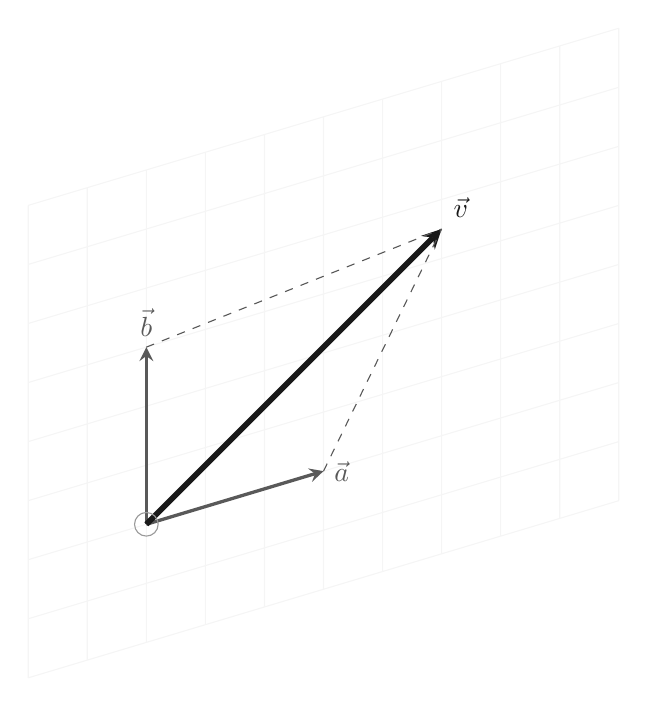
\begin{tikzpicture}[scale=1.5, >=stealth]
            \begin{scope}[cm={1,0.3,0,1,(0,0)}]
                \draw[lightGray, step=0.5] (-1,-1) grid (4,3);
            \end{scope}
            \coordinate (O) at (0,0);
            \draw[->, very thick, subGray] (O) -- (1.5, 0.45) node[right] {$\vec{a}$};
            \draw[->, very thick, subGray] (O) -- (0, 1.5) node[above] {$\vec{b}$};
            \draw[->, line width=2pt, mainBlack] (O) -- (2.5, 2.5) node[above right] {$\vec{v}$};
            \draw[dashed, subGray] (1.5, 0.45) -- (2.5, 2.5);
            \draw[dashed, subGray] (0, 1.5) -- (2.5, 2.5);
            \draw[borderGray, thin] (O) circle (0.1);
        \end{tikzpicture}
        
        \vfill
        {\large \textbf{Class:} 2年 \underline{\hspace{3em}} 組 \quad \textbf{Name:} \underline{\hspace{12em}}}
        \vspace{2cm}
    \end{center}
\end{titlepage}

% =======================================================
% 挿絵 (Art Page)
% =======================================================
\newpage
\thispagestyle{empty}
\vspace*{\fill}

\begin{center}
    \begin{tikzpicture}[scale=1.5]
        \foreach \r in {1, 2, 3} {
            \draw[lightGray, thin] (0,0) circle (\r);
        }
        \foreach \i in {1,...,8} {
            \pgfmathsetmacro{\x}{rand*2.5}
            \pgfmathsetmacro{\y}{rand*2}
            \pgfmathsetmacro{\ang}{45 + rand*15} 
            \draw[->, >=stealth, subGray, opacity=0.4] (\x, \y) -- ++(\ang:1.2);
        }
        \draw[->, >=stealth, mainBlack, line width=1.5pt] (-1, -0.5) -- ++(45:2.5) node[midway, above left, fill=white, inner sep=2pt] {\small \textbf{Will}};
        
        \node[align=center, font=\sffamily\color{mainBlack}, yshift=-4.5cm] at (0,0) {
            \small \itshape
            ``Direction matters more than location.''\\
            \vspace{0.8em}
            \footnotesize \color{subGray}
            ベクトルは「どこにいるか」を問わない。\\
            問われるのは「どこへ向かうか」という意志だけだ。
        };
    \end{tikzpicture}
\end{center}
\vspace*{\fill}

% =======================================================
% 目次
% =======================================================
\newpage
\setcounter{tocdepth}{2}
\tableofcontents
\newpage

% =======================================================
% 第1回
% =======================================================
\setcounter{section}{0} % 第1回から開始
\setKey{Freedom from Coordinates}

\section{矢印という名の自由 —— ベクトルの定義}

% -------------------------------------------------------
% 1ページ目:導入と定義
% -------------------------------------------------------
\subsection*{Prologue: 風の正体}

放課後の屋上。フェンス越しに街を見下ろしていると、友人が目を閉じて深呼吸をした。
今日はやけに風が強い。

\talk{友人}{「……北北西、風速5メートルってところかな」}
\talk{私}{「何それ、気象予報士にでもなったつもり?」}
\talk{友人}{「いや、肌で感じるんだよ。風って不思議だと思わない? 目には見えない空気の塊なのに、『こっちに向かってこれくらいの強さで吹いてる』ってことだけは、はっきりと分かる」}

私は友人の真似をして、風に意識を向けてみる。確かに、体にぶつかる圧力と、髪がなびく方向。その二つの情報だけで、私たちは「風」を認識している。

\talk{私}{(……向きと、強さ。言われてみれば、風を説明するのに『場所』は関係ない気がする。ここで吹いている風も、校庭の隅で吹いている風も、もし向きと強さが同じなら『同じ風』と呼んでいいはずだ)}

\talk{友人}{「ねえ、もしこの風を紙に書くとしたら、どう書く?」}
\talk{私}{「そりゃ、矢印でしょ。天気図とかでよくあるやつ」}
\talk{友人}{「だよね。でもさ、その矢印、地図の『どこ』に書く? 東京? それとも横浜?」}
\talk{私}{「どこでもいいんじゃないか? 『関東地方に北風』なら、関東のどこに書いても意味は通じる」}

ふと、背後から足音がした。いつの間にか先生が立っていた。

\talk{先生}{「良い議論ですね。『どこに書いても意味は同じ』。その感覚こそが、今日学ぶ新しい数学の扉を開く鍵です」}
\talk{私}{「先生……また盗み聞きですか」}
\talk{先生}{「人聞きが悪い。風の音を聞きに来ただけですよ。さて、君たちが直感的に捉えた『場所を無視して、向きと大きさだけで決まる量』。それを数学では\textbf{ベクトル}と呼びます」}

\vspace{1em}
\hrule
\vspace{2em}

\subsection{Topic 1: 住所を持たない量}

教室に戻ると、先生は黒板の左端と右端に、それぞれ一本ずつ矢印を描いた。
長さはチョーク2本分くらい。向きはどちらも斜め右上45度くらいだ。

\talk{先生}{「さて、この二つの矢印、$\vec{a}$ と $\vec{b}$ は、同じものですか? 違うものですか?」}
\talk{私}{「場所が全然違います。黒板の右と左ですから、座標で言えば別物です」}
\talk{友人}{「でも先生、さっきの風の話で言えば『同じ』だよね。向きも長さも一緒だし」}

先生はニヤリと笑って、$\vec{a}$ と $\vec{b}$ の間に大きなイコール記号を書いた。

\[ \vec{a} = \vec{b} \]

\talk{先生}{「ベクトルにとって、場所(始点の位置)は飾りです。重要なのは『どの向きに、どれだけ進むか』という性質だけ。だから、この二つは\textbf{完全に等しい}とみなします」}

\begin{SolidBox}
    \textbf{定義:ベクトル (Vector)} \\
    「大きさ(長さ)」と「向き」だけを持つ量。
    始点がどこにあっても、大きさと向きが等しければ、それらは\textbf{等しいベクトル}である。
    \[ \vec{a} = \vec{b}\longleftrightarrow \text{大きさが等しく、向きも同じ} \]
    (※ 平行移動して重なる矢印はすべて同じものとみなす)
\end{SolidBox}

\talk{私}{(……違和感がある。今まで習ってきた数学では、位置こそが絶対だった。座標 $(1,1)$ と $(2,2)$ は絶対に違う点だし、グラフ上の点Pと点Qは別物だ。それを『同じ』と言い切ってしまうなんて、なんだか乱暴すぎないか?)}

私の困惑を察したのか、友人が補足を入れる。

\talk{友人}{「ほら、RPGのゲームでさ、『北に3歩進む』っていうコマンドがあるじゃん? あれを『宿屋』で使っても『洞窟』で使っても、主人公の動き自体は同じだよね。ベクトルって、その『コマンド(命令)』のことなんじゃない?」}
\talk{私}{「あー……なるほど。物体そのものじゃなくて、『移動』というアクションを指してるのか」}

\begin{center}
\begin{tikzpicture}[scale=1.2, >=stealth]
    % Grid
    \draw[lightGray, thin] (0,0) grid (6,3);
    
    % Vectors
    \draw[->, very thick, mainBlack] (1,0.5) -- (3,1.5) node[midway, above left] {$\vec{a}$};
    \draw[->, very thick, mainBlack] (4,1.5) -- (6,2.5) node[midway, below right] {$\vec{b}$};
    
    % Equality
    \node at (3.5, 1.5) {\Huge $=$};
    
    % Description
    \node[align=center, font=\small, color=subGray] at (3.5, 0.5) {始点が違っても\\ベクトルとしては等しい};
\end{tikzpicture}
\end{center}

\talk{先生}{「その通りです。座標が『住所』なら、ベクトルは『旅』です。どこから出発しても、同じ旅は同じ旅。この自由さが、図形問題を解くときに強力な武器になるのです」}

\newpage

% -------------------------------------------------------
% 2ページ目:加法(足し算)
% -------------------------------------------------------
\subsection{Topic 2: 寄り道の算術(加法)}

\talk{先生}{「矢印が『移動』を表すなら、当然、計算もできるはずです。まずは足し算を考えてみましょう」}
\talk{友人}{「移動の足し算か……。A地点からB地点に行って、続けてBからC地点に行く、みたいな?」}

友人はノートに三角形を描き始めた。

\begin{center}
\begin{tikzpicture}[scale=1.0, >=stealth]
    \coordinate (A) at (0,0);
    \coordinate (B) at (3,1);
    \coordinate (C) at (2,2.5);
    
    \draw[->, thick, mainBlack] (A) -- (B) node[midway, below] {$\vec{a}$ (第1移動)};
    \draw[->, thick, mainBlack] (B) -- (C) node[midway, right] {$\vec{b}$ (第2移動)};
    
    \fill (A) circle (2pt) node[left] {A};
    \fill (B) circle (2pt) node[right] {B};
    \fill (C) circle (2pt) node[above] {C};
\end{tikzpicture}
\end{center}

\talk{私}{「$\vec{a} + \vec{b}$ ってことか。でもこれ、単純に長さを足すわけにはいかないよな。寄り道してる分、距離は長くなってるし」}
\talk{先生}{「ベクトルが重視するのは『プロセス』ではなく、最終的な『結果』です。Aから出発して、最終的にどこに着きましたか?」}
\talk{私}{「Cです」}
\talk{先生}{「ならば、ベクトルの世界では『AからCへ直接移動した』のと等しいと考えます」}

先生はAからCへ、点線で力強い矢印を引いた。

\begin{center}
\begin{tikzpicture}[scale=1.0, >=stealth]
    \coordinate (A) at (0,0);
    \coordinate (B) at (3,1);
    \coordinate (C) at (2,2.5);
    
    \draw[->, thick, subGray] (A) -- (B) node[midway, below] {$\vec{a}$};
    \draw[->, thick, subGray] (B) -- (C) node[midway, right] {$\vec{b}$};
    \draw[->, very thick, mainBlack] (A) -- (C) node[midway, above left] {$\vec{a}+\vec{b}$};
    
    \node[align=left, font=\small] at (4, 1.5) {寄り道(プロセス)は無視!\\ 結果(Start $\to$ Goal)だけを見る};
\end{tikzpicture}
\end{center}

\talk{私}{(なるほど……。どんなに苦労して山道を登っても($\vec{a}+\vec{b}$)、ヘリコプターで直行しても($\vec{c}$)、位置の変化としては同じ。ベクトルってやつは、随分とドライで結果主義な性格なんだな)}

\begin{NoteBox}
    \textbf{ベクトルの和(三角形の法則)}
    \[ \overrightarrow{\text{AB}} + \overrightarrow{\text{BC}} = \overrightarrow{\text{AC}} \]
    しりとりのように「終点」と「次の始点」が繋がっているとき、最初と最後を直接結ぶ矢印が「和」となる。
\end{NoteBox}

\talk{友人}{「ねえ、これって逆でもいいよね? 先に $\vec{b}$ 進んでから、$\vec{a}$ 進んでも……」}
\talk{先生}{「やってみましょうか」}

友人は図に平行四辺形を描き足した。Aから $\vec{b}$ の方向に進み、そこから $\vec{a}$ の方向に進む。……たどり着く先は、やはり点Cだ。

\begin{center}
\begin{tikzpicture}[scale=0.8, >=stealth]
    \coordinate (A) at (0,0);
    \coordinate (B) at (3,1);
    \coordinate (D) at (-1, 1.5);
    \coordinate (C) at (2, 2.5);
    
    \draw[->, thick, mainBlack] (A) -- (B) node[midway, below] {$\vec{a}$};
    \draw[->, thick, mainBlack] (B) -- (C) node[midway, right] {$\vec{b}$};
    
    \draw[->, thick, dashed] (A) -- (D) node[midway, left] {$\vec{b}$};
    \draw[->, thick, dashed] (D) -- (C) node[midway, above] {$\vec{a}$};
    
    \draw[->, very thick, mainBlack] (A) -- (C) node[midway, right, fill=white, inner sep=1pt] {$\vec{a}+\vec{b}$};
    
    \node at (1, -1) {$\vec{a}+\vec{b} = \vec{b}+\vec{a}$ (交換法則)};
\end{tikzpicture}
\end{center}

\talk{友人}{「やっぱり! 順番を変えても結果は同じ。普通の足し算と同じで『交換法則』が成り立つんだ」}
\talk{先生}{「素晴らしい。これを\textbf{平行四辺形の法則}とも呼びます。力が合わさるとき(合力)のイメージですね」}

\newpage

% -------------------------------------------------------
% 3ページ目:減法(引き算)
% -------------------------------------------------------
\subsection{Topic 3: 逆再生の矢印(減法)}

\talk{私}{「足し算がこれだけ直感的だと、引き算が怖くなりますね。$\vec{a} - \vec{b}$ って、イメージしづらいです」}
\talk{友人}{「引き算って、数学では『負の数を足す』ことだよね。$3 - 5 = 3 + (-5)$ みたいに」}
\talk{先生}{「その発想でいきましょう。ベクトルにおける『マイナス』とは何だと思いますか?」}
\talk{私}{「プラスが『進む』なら、マイナスは『戻る』……つまり、逆向きの矢印ですか?」}

先生は頷き、黒板に $\vec{b}$ と正反対の向きを持つ矢印 $-\vec{b}$ を描いた。

\begin{SolidBox}
    \textbf{逆ベクトル} \\
    ベクトル $\vec{a}$ に対して、大きさは同じで向きが反対のベクトルを $-\vec{a}$ と書く。
\end{SolidBox}

\talk{先生}{「では、$\vec{a} - \vec{b}$ を $\vec{a} + (-\vec{b})$ と考えて作図してみましょう」}

私はノートの上で手を動かす。
まず $\vec{a}$ を描く。その終点から、$\vec{b}$ を\textbf{逆向きに}継ぎ足す。

\begin{center}
\begin{tikzpicture}[scale=1.0, >=stealth]
    \coordinate (O) at (0,0);
    \coordinate (A) at (3,0.5); % vec a
    \coordinate (B) at (1,2);   % vec b
    
    % Step 1: a + (-b)
    \begin{scope}[shift={(0,0)}]
        \draw[->, thick, subGray] (0,0) -- (3,0.5) node[midway, below] {$\vec{a}$};
        \draw[->, thick, subGray] (3,0.5) -- (2,-1.5) node[midway, right] {$-\vec{b}$};
        \draw[->, thick, dashed] (0,0) -- (2,-1.5) node[midway, left] {$\vec{a}-\vec{b}$};
        \node at (1.5, -2.5) {考え方A:足し算に直す};
    \end{scope}
    
    % Step 2: Triangle difference
    \begin{scope}[shift={(6,-1)}]
        \coordinate (OO) at (0,0);
        \coordinate (AA) at (3,0.5);
        \coordinate (BB) at (1,2);
        
        \draw[->, thick, subGray] (OO) -- (AA) node[midway, below] {$\vec{a}$};
        \draw[->, thick, subGray] (OO) -- (BB) node[midway, left] {$\vec{b}$};
        \draw[->, very thick, mainBlack] (BB) -- (AA) node[midway, above right] {$\vec{a}-\vec{b}$};
        
        \fill (OO) circle (1.5pt) node[below left] {O};
        \fill (AA) circle (1.5pt) node[right] {A};
        \fill (BB) circle (1.5pt) node[left] {B};
        \node at (1.5, -1.5) {考え方B:始点を揃える};
    \end{scope}
\end{tikzpicture}
\end{center}

\talk{私}{「……描けましたけど、なんか変な場所に矢印ができちゃいました」}
\talk{先生}{「では、その矢印を平行移動して、始点を $\vec{a}, \vec{b}$ の始点(O)と合わせてみてください。……おや? もっと簡単な見方がありませんか?」}

友人が図をじっと見つめ、ハッとした顔をする。

\talk{友人}{「これ、$\vec{b}$ の先っちょから、$\vec{a}$ の先っちょに向かう矢印と同じじゃない?」}
\talk{私}{「本当だ! 三角形の残りの一辺になってる」}

\talk{私}{(待てよ……。$\vec{a}-\vec{b}$ という計算結果が、BからAへの矢印($\overrightarrow{\text{BA}}$)になる。これって『A 引く B』なのに、矢印は『B から A』へ向かっている。順序が逆に見えるな)}

\talk{先生}{「その気付きは鋭いですね。$\vec{a}-\vec{b}$ は、\textbf{『終点(A) - 始点(B)』}を表しているのです。式で書くとこうなります」}

\begin{SolidBox}
    \textbf{ベクトルの差(視点の変更)}
    \[ \overrightarrow{\text{OA}} - \overrightarrow{\text{OB}} = \overrightarrow{\text{BA}} \]
    \textbf{「あとひくまえ」}(後ろのAから、前のBを引く)と覚える。
    これは、基準点Oから見た「差」が、BからAを見る相対的なベクトルになることを意味する。
\end{SolidBox}

\talk{私}{(BからAを見る……。つまり、引き算というのは「視点の移動」なのか。Oから見ていた世界を、Bからの視点に書き換える。それがベクトルの引き算の本質なのかもしれない)}

\newpage

% -------------------------------------------------------
% 4ページ目:練習問題・エピローグ
% -------------------------------------------------------
\subsection*{Check: 理解度の確認}

\begin{NoteBox}
    \textbf{問題} \\
    正六角形ABCDEFにおいて、中心をOとする。
    $\overrightarrow{\text{AB}} = \vec{a}, \overrightarrow{\text{AF}} = \vec{b}$ とするとき、次のベクトルを $\vec{a}, \vec{b}$ で表せ。
    \begin{enumerate}
        \item $\overrightarrow{\text{AO}}$
        \item $\overrightarrow{\text{AC}}$
        \item $\overrightarrow{\text{BF}}$
    \end{enumerate}
\end{NoteBox}

\talk{友人}{「うわ、六角形か。ちょっと複雑そう」}
\talk{私}{「でも、パズルみたいに分解すればいけるはずだ。$\vec{a}$ と $\vec{b}$ の組み合わせで道を作ればいい」}

\begin{center}
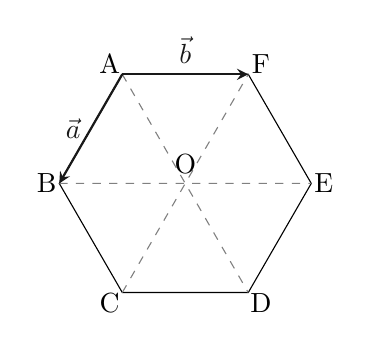
\begin{tikzpicture}[scale=0.8, >=stealth]
    \coordinate (A) at (-1, 1.732);
    \coordinate (B) at (-2, 0);
    \coordinate (C) at (-1, -1.732);
    \coordinate (D) at (1, -1.732);
    \coordinate (E) at (2, 0);
    \coordinate (F) at (1, 1.732);
    \coordinate (O) at (0,0);
    
    \draw (A)--(B)--(C)--(D)--(E)--(F)--cycle;
    \draw[dashed, gray] (A)--(D) (B)--(E) (C)--(F);
    
    \draw[->, thick, mainBlack] (A) -- (B) node[midway, left] {$\vec{a}$};
    \draw[->, thick, mainBlack] (A) -- (F) node[midway, above] {$\vec{b}$};
    
    \node at (0, 0.3) {O};
    \node at (-1.2, 1.9) {A}; \node at (-2.2, 0) {B}; \node at (-1.2, -1.9) {C};
    \node at (1.2, -1.9) {D}; \node at (2.2, 0) {E}; \node at (1.2, 1.9) {F};
\end{tikzpicture}
\end{center}

\talk{私}{「(1) $\overrightarrow{\text{AO}}$ は……図を見ると、これ $\vec{a}$ と $\vec{b}$ の平行四辺形の対角線じゃないか?」}
\talk{友人}{「あ、本当だ。$\overrightarrow{\text{AB}}$ と $\overrightarrow{\text{AF}}$ の足し算になってる。つまり $\vec{a} + \vec{b}$ だね」}

\talk{私}{「(2) $\overrightarrow{\text{AC}}$ は? AからCへ行くには、A$\to$B$\to$Cと進めばいい。$\overrightarrow{\text{AB}}$ は $\vec{a}$ だけど、$\overrightarrow{\text{BC}}$ は?」}
\talk{友人}{「$\overrightarrow{\text{BC}}$ って、向きと長さを見ると $\overrightarrow{\text{AO}}$ と同じだよ。さっき求めた $\vec{a}+\vec{b}$ が使える!」}
\talk{私}{「なるほど! じゃあ $\vec{a} + (\vec{a}+\vec{b}) = 2\vec{a} + \vec{b}$ か」}

\talk{私}{「最後の (3) $\overrightarrow{\text{BF}}$ は……BからFへ。これは引き算が使えそうだな」}
\talk{友人}{「始点をAに揃えちゃおうよ。『あとひくまえ』で $\overrightarrow{\text{AF}} - \overrightarrow{\text{AB}}$ になるから……」}
\talk{私}{「$\vec{b} - \vec{a}$ 。一瞬で出たな」}

\subsection*{Epilogue: 自由を手にして}

問題を解き終えると、屋上の風は少し穏やかになっていた。

\talk{先生}{「どうですか? ベクトルという新しい眼鏡を通すと、図形が少し違って見えませんか?」}
\talk{私}{「はい。なんていうか……図形が『形』じゃなくて『道順』に見えてきました。どんなに複雑な場所でも、矢印を継ぎ足していけば辿り着けるような」}
\talk{友人}{「僕は計算ができるのが嬉しいな。図形の問題って『ひらめき』が必要で苦手だったけど、ベクトルなら『始点引く終点』とか、ルール通りにやれば答えが出る」}

先生は満足そうに頷いた。

\talk{先生}{「その感覚を大切にしてください。今日は『1本だけの矢印』の話でしたが、次回は『2本の矢印』が作る世界——平面全体を支配する方法について学びましょう」}

\vspace{1em}
\begin{flushright}
    \textit{To be continued in Lecture 2...}
\end{flushright}

\newpage

% =======================================================
% 第2回
% =======================================================
\setcounter{section}{1} % 第2回
\setKey{The Fabric of the Plane}

\section{平面を支配する二つの矢 —— 一次独立}

% -------------------------------------------------------
% 1ページ目:プロローグ(1次元の限界)
% -------------------------------------------------------
\subsection*{Prologue: 線路と野原}

グラウンドの白いラインの上を、友人が綱渡りのようにバランスを取りながら歩いている。
彼はふと立ち止まり、足元を見つめたまま呟いた。

\talk{友人}{「ねえ、ベクトルが1本しかない世界って、すごく窮屈だと思わない?」}
\talk{私}{「窮屈? ……どういうこと?」}
\talk{友人}{「だってさ、手元に $\vec{a}$ しかなかったら、前($2\vec{a}$)に進むか、後ろ($-1\vec{a}$)に戻るかしかできないでしょ。どんなに頑張っても、この白線(直線)からは絶対に出られないんだよ」}

私は彼にならって、白線の上を歩いてみた。確かに、どれだけ係数 $k$ を変えて $k\vec{a}$ と計算したところで、それは単なる「伸縮」にすぎない。

\talk{私}{(……言われてみればそうだね。1本だけの矢印は、無限に長い『線路』みたいなものだ。僕たちはそのレールの上に縛り付けられている)}

\talk{私}{「確かに。1本だけだと『1次元』の世界に閉じ込められちゃうね。自由度がないっていうか」}
\talk{友人}{「でもさ、もしもう1本、違う向きの矢印 $\vec{b}$ があったら……」}

友人は突然、白線から勢いよく飛び降りて、グラウンドの芝生を斜めに走り出した。

\talk{友人}{「ほら! 右にも行けるし、斜めにも行ける。この広いグラウンド(平面)のどこへでも行ける気がしない?」}

芝生の上で振り返った友人の笑顔を見て、私はハッとした。
線路(直線)から野原(平面)へ。次元が一つ上がるというのは、こういう開放感のことなのかもしれない。

\vspace{1em}
\hrule
\vspace{2em}

\subsection{Topic 1: 意味のある追加、無意味な追加}

先生がゆっくりと歩いてきた。私たちの遊びを咎める様子はなく、むしろ面白がっているようだ。

\talk{先生}{「その直感は正しいですよ。次元を広げるには、新しいベクトルが必要です。しかし、ただ『2本あればいい』というわけではありません。例えば……」}

先生はしゃがみ込み、地面に描かれた白線($\vec{a}$)の上に、チョークでもう一本、ぴったり重なるように矢印を描き足した。

\talk{先生}{「これで矢印は2本になりました。さて、行ける場所は増えましたか?」}
\talk{私}{「あ、それじゃ意味ないよ。$\vec{a}$ と同じ向きの $\vec{b}$ を足しても、結局同じ線の上しか動けないし」}

\talk{私}{(線路の上に、もう一台電車を置いたようなものだ。連結したって、行ける場所は変わらない。新しい世界に行くには、既存のレールから『脱線』する勇気が必要なんだ)}

\talk{友人}{「あと、$\vec{0}$(ゼロベクトル)もダメだね。動かない矢印をもらっても嬉しくないし」}
\talk{先生}{「その通り。新しい次元へ飛び出すためには、既存の矢印とは『質的に違う』矢印が必要です。これを数学の言葉で定義してみましょう」}

\begin{SolidBox}
    \textbf{定義:一次独立(Linear Independence)} \\
    2つのベクトル $\vec{a}, \vec{b}$ が、以下の条件を満たすとき、それらは\textbf{一次独立}であるという。
    \[ \vec{a} \neq \vec{0}, \quad \vec{b} \neq \vec{0}, \quad \vec{a} \not\parallel \vec{b} \]
    \begin{itemize}
        \item $\vec{0}$ ではない(大きさがある)
        \item 平行ではない(向きが異なる)
    \end{itemize}
    この条件が揃って初めて、2本の矢印は「平面」を織りなすことができる。
\end{SolidBox}

\newpage

% -------------------------------------------------------
% 2ページ目:分解の原理
% -------------------------------------------------------
\subsection{Topic 2: 歪んだグリッド(分解)}

\talk{友人}{「ねえ、一次独立な2本($\vec{a}, \vec{b}$)があれば、本当に行けない場所はないのかな? 平面の果てまで行ける?」}
\talk{私}{「試してみようよ。例えば……あそこのポール(点P)まで行きたいとするね」}

私はノートを開き、点Pと、手元にある2本の矢印を描いた。
$\vec{a}$ は真横、$\vec{b}$ は斜め上。直交していない、ちょっと使いにくそうな矢印たちだ。

\talk{私}{「この2本だけでPに行けるかな? クレーンゲームみたいに考えてみよう」}

私はペン先を動かしてシミュレーションする。

\talk{私}{「まず $\vec{a}$ 方向にグイーッと進んで……Pの真下あたりまで行く。でも $\vec{b}$ が斜めだから、真上に上がれないな」}
\talk{友人}{「逆だよ。先に $\vec{b}$ の平行線を引いてみればいいんじゃない?」}

友人がノートに補助線を引く。$\vec{a}$ の延長線と、Pを通って $\vec{b}$ に平行な線。その交差点が見えてきた。

\talk{私}{「なるほど! $\vec{a}$ でここまで進んで、そこから $\vec{b}$ 方向に修正すれば……ほら、着いた」}

\begin{center}
\begin{tikzpicture}[scale=1.0, >=stealth]
    \coordinate (O) at (0,0);
    \coordinate (A) at (2,0.5);
    \coordinate (B) at (1,2);
    \coordinate (P) at (3.8, 2.35);
    
    % Grid
    \draw[lightGray] (0,0) -- (4,1);
    \draw[lightGray] (0,0) -- (2,4);
    \draw[dashed, subGray] (O) -- (3, 0.75) node[below] {$s\vec{a}$};
    \draw[dashed, subGray] (3, 0.75) -- (P) node[right] {$t\vec{b}$};
    
    \draw[->, thick, mainBlack] (O) -- (A) node[below] {$\vec{a}$};
    \draw[->, thick, mainBlack] (O) -- (B) node[left] {$\vec{b}$};
    \draw[->, very thick, mainBlack] (O) -- (P) node[above right] {$\vec{p}$};
    
    \fill (O) circle (1.5pt) node[below left] {O};
    \fill (P) circle (1.5pt) node[above] {P};
    
    \node[align=left, font=\small, color=subGray] at (5, 1) {斜めに進んでから\\斜めに上がる};
\end{tikzpicture}
\end{center}

\talk{私}{(まるで、軸が歪んだグラフ用紙だ。普通のマス目は正方形だけど、この世界では平行四辺形のマス目が広がっている。……でも、マス目が歪んでいても『右に3マス、上に2マス』みたいに数えられることに変わりはないんだ)}

\talk{先生}{「良い図が描けましたね。それがベクトルの\textbf{分解}です。そして、最も大事なことは何だと思いますか?」}
\talk{私}{「えっと……必ずたどり着けること?」}
\talk{先生}{「それもですが、\textbf{行き方が一通りしかない}ということです」}

\begin{SolidBox}
    \textbf{分解の一意性} \\
    $\vec{a}, \vec{b}$ が一次独立ならば、任意のベクトル $\vec{p}$ は
    \[ \vec{p} = s\vec{a} + t\vec{b} \]
    という形で\textbf{ただ1通り}に表せる。
\end{SolidBox}

\talk{友人}{「そっか。もし行き方が二通りあったら、住所が決まらなくて迷子になっちゃうもんね」}
\talk{私}{「『係数比較』ができるのも、このルールのおかげなんだね」}

\begin{NoteBox}
    \textbf{係数比較の原理} \\
    $\vec{a}, \vec{b}$ が一次独立のとき、
    \[ s\vec{a} + t\vec{b} = s'\vec{a} + t'\vec{b} \iff s=s' \text{ かつ } t=t' \]
    ベクトルの等式を、連立方程式(係数の等式)に持ち込める。
\end{NoteBox}

\newpage

% -------------------------------------------------------
% 3ページ目:練習問題(六角形)
% -------------------------------------------------------
\subsection*{Check: 迷路を解くように}

先生が黒板に正六角形を描いた。

\begin{NoteBox}
    \textbf{問題} \\
    正六角形ABCDEFにおいて、中心をOとする。
    $\overrightarrow{\text{AB}} = \vec{a}, \overrightarrow{\text{AF}} = \vec{b}$ とするとき、次のベクトルを $\vec{a}, \vec{b}$ で表せ。
    \begin{enumerate}
        \item $\overrightarrow{\text{AO}}$
        \item $\overrightarrow{\text{AC}}$
        \item $\overrightarrow{\text{BF}}$
    \end{enumerate}
\end{NoteBox}

\talk{友人}{「うわ、六角形か。線がいっぱいで複雑そう……」}
\talk{私}{「でもさっきの話だと、$\vec{a}$ と $\vec{b}$ さえあればどこへでも行けるはずだよ。パズルみたいに分解してみよう」}

\begin{center}
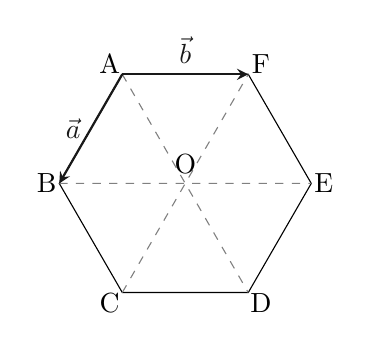
\begin{tikzpicture}[scale=0.8, >=stealth]
    \coordinate (A) at (-1, 1.732);
    \coordinate (B) at (-2, 0);
    \coordinate (C) at (-1, -1.732);
    \coordinate (D) at (1, -1.732);
    \coordinate (E) at (2, 0);
    \coordinate (F) at (1, 1.732);
    \coordinate (O) at (0,0);
    
    \draw (A)--(B)--(C)--(D)--(E)--(F)--cycle;
    \draw[dashed, gray] (A)--(D) (B)--(E) (C)--(F);
    
    \draw[->, thick, mainBlack] (A) -- (B) node[midway, left] {$\vec{a}$};
    \draw[->, thick, mainBlack] (A) -- (F) node[midway, above] {$\vec{b}$};
    
    \node at (0, 0.3) {O};
    \node at (-1.2, 1.9) {A}; \node at (-2.2, 0) {B}; \node at (-1.2, -1.9) {C};
    \node at (1.2, -1.9) {D}; \node at (2.2, 0) {E}; \node at (1.2, 1.9) {F};
\end{tikzpicture}
\end{center}

\talk{私}{「まず (1) $\overrightarrow{\text{AO}}$ だけど……図を見ると、これって平行四辺形 ABOF の対角線になってない?」}
\talk{友人}{「あ、本当だ! $\overrightarrow{\text{AB}}$ と $\overrightarrow{\text{AF}}$ の足し算でいけるね。つまり $\vec{a} + \vec{b}$ だ」}

\talk{私}{「次は (2) $\overrightarrow{\text{AC}}$ 。AからCへ行くには、A$\to$B$\to$Cって進めばいいよね。$\overrightarrow{\text{AB}}$ は $\vec{a}$ だけど、$\overrightarrow{\text{BC}}$ はどう表せばいい?」}

私は図の中の $\overrightarrow{\text{BC}}$ を指でなぞる。向きは右下。長さは……。

\talk{私}{(……あれ? この矢印、さっき求めた $\overrightarrow{\text{AO}}$ と全く同じじゃないか? 平行移動すれば重なる!)}

\talk{友人}{「$\overrightarrow{\text{BC}}$ って、$\overrightarrow{\text{AO}}$ と同じベクトルだよね! さっきの答えが使えるよ」}
\talk{私}{「なるほど! じゃあ $\vec{a} + (\vec{a}+\vec{b})$ で、$2\vec{a} + \vec{b}$ になるわけか」}

\talk{私}{(過去に求めた答えが、次の移動のパーツになる。RPGで手に入れたアイテムを使って新しいエリアに進むみたいだ)}

\talk{私}{「最後の (3) $\overrightarrow{\text{BF}}$ は……BからFへ。Aを経由すると遠回りだけど、どう計算する?」}
\talk{友人}{「『あとひくまえ』が使えるんじゃない? 始点をAに揃えちゃえば計算だけでいけるよ」}
\talk{私}{「そうか、$\overrightarrow{\text{AF}} - \overrightarrow{\text{AB}}$ だから、$\vec{b} - \vec{a}$ 。……一瞬で出たな」}

\newpage

% -------------------------------------------------------
% 4ページ目:エピローグ
% -------------------------------------------------------
\subsection*{Epilogue: 自由の地図}

問題を解き終える頃には、グラウンドには夕日が差し込んでいた。

\talk{私}{「なんか不思議だね。あんなに複雑な六角形の中を歩き回ったのに、使ったのはたった2種類の矢印だけだったなんて」}
\talk{友人}{「うん。どんな場所でも、$\vec{a}$ と $\vec{b}$ の組み合わせだけで住所が書けるんだね。これなら宇宙の果てまで迷子にならなそう」}

\talk{私}{(歪んだ世界でも、基準さえしっかりしていれば、迷わず目的地にたどり着ける。一次独立という条件は、僕たちに『座標』という地図を与えてくれたんだ)}

先生がノートを覗き込んで、優しく微笑んだ。

\talk{先生}{「よく理解できていますね。君たちはいま、平面という広大な世界を、たった2本の矢印で支配する方法を学んだのです」}
\talk{私}{「支配、ですか。なんか大げさですね」}
\talk{先生}{「ふふ、でも本当のことでしょう? 次回は、この矢印を『成分(数字)』に翻訳して、もっと精密に計算する方法を学びましょう。分度器も定規もいらない、魔法のような計算の世界ですよ」}

\vspace{2em}
\begin{flushright}
    \textit{To be continued in Lecture 3...}
\end{flushright}

\newpage

% =======================================================
% 第3回
% =======================================================
\setcounter{section}{2} % 第3回
\setKey{Translation to Numbers}

\section{数の架け橋 —— 成分表示}

% -------------------------------------------------------
% 1ページ目:プロローグと標準基底
% -------------------------------------------------------
\subsection*{Prologue: 最も贅沢な基底}

教室に戻ると、友人が机の上に方眼紙(グラフ用紙)を広げていた。
見慣れた正方形のマス目が、整然と並んでいる。

\talk{友人}{「ねえ、さっきは斜めに歪んだマス目(一次独立な $\vec{a}, \vec{b}$)の話をしたけどさ。結局のところ、僕らが一番使い慣れてるのってこれだよね」}
\talk{私}{「方眼紙か。確かに、直角に交わってるし、目盛りも $1$ ずつだし、安心感があるね」}

私は方眼紙の太線を指でなぞる。横線と縦線。
前回学んだ「一次独立」な2本の矢印として、あえてこの「横向きの1目盛り」と「縦向きの1目盛り」を選んだらどうなるだろう?

\talk{私}{(……歪んだグリッドでも住所は特定できた。でも、もしグリッドが正方形なら、計算はもっと簡単になるはずだ。この特別な2本には、何か名前があるのかな)}

先生が背後から声をかけた。

\talk{先生}{「おや、良いところに目をつけましたね。その『長さ1で直行する2本』は、数学の世界で最も贅沢で、最も標準的な基底です」}
\talk{友人}{「贅沢?」}
\talk{先生}{「ええ。計算の手間を極限まで減らしてくれますからね。これを\textbf{基本ベクトル}と呼び、$\vec{e}_1, \vec{e}_2$ で表します」}

\begin{center}
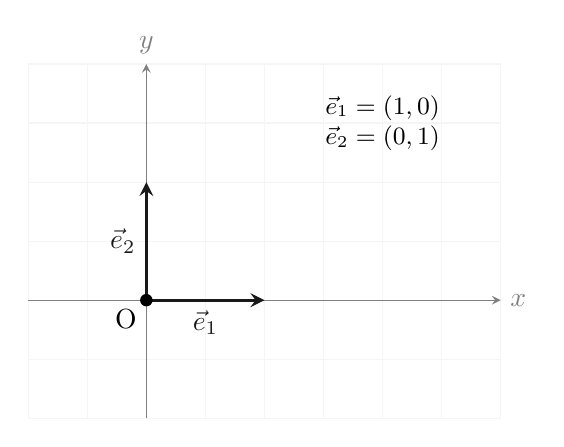
\begin{tikzpicture}[scale=1.5, >=stealth]
    % Grid
    \draw[lightGray, step=0.5] (-1,-1) grid (3,2);
    \draw[->, gray] (-1,0) -- (3,0) node[right] {$x$};
    \draw[->, gray] (0,-1) -- (0,2) node[above] {$y$};
    
    % Basis Vectors
    \draw[->, very thick, mainBlack] (0,0) -- (1,0) node[midway, below] {$\vec{e}_1$};
    \draw[->, very thick, mainBlack] (0,0) -- (0,1) node[midway, left] {$\vec{e}_2$};
    
    \node[align=left, font=\small] at (2, 1.5) {$\vec{e}_1 = (1, 0)$ \\ $\vec{e}_2 = (0, 1)$};
    \fill (0,0) circle (1.5pt) node[below left] {O};
\end{tikzpicture}
\end{center}

\vspace{1em}
\hrule
\vspace{2em}

\subsection{Topic 1: 矢印を「数」に変える}

\talk{先生}{「さて、この特別な基底 $\vec{e}_1, \vec{e}_2$ を使えば、どんなベクトル $\vec{a}$ も分解できるはずです。例えば、右に3、上に2進むベクトルなら?」}
\talk{友人}{「それは簡単だよ。$\vec{a} = 3\vec{e}_1 + 2\vec{e}_2$ でしょ」}
\talk{先生}{「正解です。でも、毎回 $\vec{e}_1, \vec{e}_2$ と書くのは面倒ですよね? そこで、係数だけを取り出してこう書くことにします」}

\[ \vec{a} = (3, 2) \]

\talk{私}{「えっ、それって……座標の書き方と同じじゃない?」}

私は少し戸惑った。点 $A(3, 2)$ と、ベクトル $\vec{a} = (3, 2)$。見た目が全く同じだ。これじゃあ混乱してしまう。

\talk{私}{(点は「場所」を表す住所だ。ベクトルは「移動」を表す矢印だ。意味が違うのに、同じ記号を使っていいのか? ……いや、待てよ。原点Oから出発したと考えれば、矢印の先っちょは点Aに重なるな)}

\talk{先生}{「良い疑問です。確かに見た目は同じですが、意味が異なります」}

\begin{SolidBox}
    \textbf{定義:成分表示 (Component Representation)} \\
    ベクトル $\vec{a}$ を $\vec{a} = (a_1, a_2)$ と書くとき、それは
    「$x$軸方向に $a_1$、$y$軸方向に $a_2$ 進め」という\textbf{命令(移動量)}を表す。
\end{SolidBox}

\talk{友人}{「なるほど。座標の $(3, 2)$ は『ここ』っていう一点を指すけど、ベクトルの $(3, 2)$ は『右に3、上に2』っていう動きを指すんだね」}
\talk{私}{「だから、始点がどこにあっても $(3, 2)$ は $(3, 2)$ なんだ。……納得したよ」}

\begin{center}
\begin{tikzpicture}[scale=1.0, >=stealth]
    \draw[lightGray] (0,0) grid (5,3);
    
    % Vector at Origin
    \draw[->, thick, mainBlack] (0,0) -- (3,1) node[midway, above left] {$\vec{a}=(3,1)$};
    \fill (3,1) circle (2pt) node[right] {点$(3,1)$};
    
    % Vector shifted
    \draw[->, thick, mainBlack] (1,1.5) -- (4,2.5) node[midway, above left] {これも $\vec{a}=(3,1)$};
    
    \node[align=center, font=\small] at (2.5, -0.5) {始点が原点なら、\\終点の座標と成分は一致する};
\end{tikzpicture}
\end{center}

\newpage

% -------------------------------------------------------
% 2ページ目:計算の導入(大きさ)
% -------------------------------------------------------
\subsection{Topic 2: 図形問題が計算問題に変わる}

\talk{友人}{「ねえ、矢印を数(成分)で書くと、何がいいことがあるの?」}
\talk{私}{「うーん、グラフ用紙に書きやすくなる……とか?」}
\talk{先生}{「もっと劇的な変化がありますよ。例えば、ベクトルの\textbf{『長さ』}を知りたいとき、定規がいらなくなります」}

先生は黒板に $\vec{a} = (3, 4)$ と書いた。

\talk{先生}{「この矢印の長さ $|\vec{a}|$ はいくつですか?」}
\talk{私}{「えっと、右に3行って、上に4上がるんだから……あ、直角三角形ができる!」}

私はノートの隅に図を描いてみる。底辺が3、高さが4の直角三角形。その斜辺がベクトルの長さだ。

\talk{私}{「三平方の定理が使えるね。$\sqrt{3^2 + 4^2} = \sqrt{9+16} = \sqrt{25}$ だから……5だ」}

\begin{NoteBox}
    \textbf{ベクトルの大きさ(長さ)}
    $\vec{a} = (a_1, a_2)$ のとき、
    \[ |\vec{a}| = \sqrt{a_1^2 + a_2^2} \]
\end{NoteBox}

\talk{私}{(これはすごいことかもしれない。今までは『図を描いて定規で測る』しかなかった長さが、ただの足し算とルートの計算だけで求まってしまった。図形の世界が、数の世界に翻訳されたんだ)}

\talk{友人}{「じゃあさ、2点間の距離も出せるんじゃない? A$(1, 2)$ から B$(4, 6)$ までの距離とか」}
\talk{私}{「AからBへの矢印 $\overrightarrow{\text{AB}}$ を作ればいいんだよ。前回やった『あとひくまえ(終点-始点)』だ」}

\[ \overrightarrow{\text{AB}} = \overrightarrow{\text{OB}} - \overrightarrow{\text{OA}} = (4, 6) - (1, 2) = (3, 4) \]

\talk{私}{「移動量は $(3, 4)$ だから、長さはさっきと同じ 5 だね」}
\talk{友人}{「うわ、中学校でやった『2点間の距離の公式』そのままだ。あれってベクトルの引き算だったんだね」}

\begin{SolidBox}
    \textbf{ベクトルの演算(成分)} \\
    $\vec{a}=(a_1, a_2), \vec{b}=(b_1, b_2)$ のとき
    \begin{itemize}
        \item \textbf{和・差}:同じ成分同士を足し引きする。
        \[ \vec{a} \pm \vec{b} = (a_1 \pm b_1, \ a_2 \pm b_2) \]
        \item \textbf{実数倍}:すべての成分を $k$ 倍する。
        \[ k\vec{a} = (ka_1, \ ka_2) \]
    \end{itemize}
\end{SolidBox}

\newpage

% -------------------------------------------------------
% 3ページ目:平行条件
% -------------------------------------------------------
\subsection{Topic 3: 向きを計算で判定する}

\talk{先生}{「長さが計算できるなら、\textbf{『向き』}も計算で判定できるはずです。例えば、二つのベクトルが\textbf{平行}かどうか、どうやって調べますか?」}
\talk{友人}{「グラフに描いてみて、傾きが同じなら平行かな」}
\talk{私}{「傾き……つまり $x$ の増加量に対する $y$ の増加量か。$\vec{a}=(a_1, a_2)$ なら $\frac{a_2}{a_1}$ だね」}

私は式変形を試みる。$\vec{a}$ と $\vec{b}$ が平行なら、傾きが等しいはずだ。
\[ \frac{a_2}{a_1} = \frac{b_2}{b_1} \]

\talk{私}{「これでもいいけど、分母が0のとき(垂直な線とか)が怖いな。分母を払って…… $a_2 b_1 = a_1 b_2$ 。これなら安全か」}
\talk{先生}{「その式、片方に寄せて整理すると美しくなりますよ」}

\[ a_1 b_2 - a_2 b_1 = 0 \]

\begin{SolidBox}
    \textbf{成分による平行条件} \\
    $\vec{a} = (a_1, a_2), \vec{b} = (b_1, b_2)$ のとき
    \[ \vec{a} \parallel \vec{b} \iff a_1 b_2 - a_2 b_1 = 0 \]
    (たすき掛けの積が等しい:$1 \times 2 - 2 \times 1 = 0$ のイメージ)
\end{SolidBox}

\talk{友人}{「へええ。図を見なくても、クロスして掛け算するだけで平行かどうかわかっちゃうんだ」}
\talk{私}{(図形の性質である『平行』が、単なる『引き算の結果が0』という数式に変わった。幾何学の問題を代数学の問題にすり替える……これがベクトルの真の力なのかもしれない)}

\begin{center}
\begin{tikzpicture}[scale=1.0, >=stealth]
    \draw[->, thick, mainBlack] (0,0) -- (2,1) node[midway, above left] {$\vec{a}(2,1)$};
    \draw[->, thick, mainBlack] (3,0) -- (7,2) node[midway, below right] {$\vec{b}(4,2)$};
    
    \node at (5, -1) {傾き $\frac{1}{2}$ と $\frac{2}{4}$ は等しい};
    \node at (5, -1.5) {$2 \times 2 - 1 \times 4 = 0$};
\end{tikzpicture}
\end{center}

\vspace{1em}
\hrule
\vspace{2em}

\subsection*{Check: 計算の練習}

先生が黒板に問題を書き出した。

\begin{NoteBox}
    \textbf{問題} \\
    $\vec{a} = (2, -1), \vec{b} = (-3, 4)$ とする。
    \begin{enumerate}
        \item $2\vec{a} + 3\vec{b}$ の成分と大きさを求めよ。
        \item $\vec{a} + t\vec{b}$ が、ベクトル $\vec{c} = (1, 2)$ と平行になるとき、実数 $t$ の値を求めよ。
    \end{enumerate}
\end{NoteBox}

\talk{友人}{「(1)は代入して計算するだけだね。$x$成分は $2(2) + 3(-3) = 4-9 = -5$。$y$成分は $2(-1) + 3(4) = -2+12 = 10$。だから $(-5, 10)$ だ」}
\talk{私}{「大きさは、$\sqrt{(-5)^2 + 10^2} = \sqrt{25+100} = \sqrt{125}$。簡単にして $5\sqrt{5}$ だね」}

\talk{友人}{「(2)は……まず $\vec{a} + t\vec{b}$ を計算しなきゃ。$(2-3t, -1+4t)$ かな」}
\talk{私}{「それが $\vec{c}=(1, 2)$ と平行になるんだから、さっきの『クロス掛け算』が使えるよ」}

私はノートに式を立てる。
\[ (2-3t) \times 2 - (-1+4t) \times 1 = 0 \]
\[ 4 - 6t + 1 - 4t = 0 \]
\[ -10t + 5 = 0 \]
\[ 10t = 5 \implies t = \frac{1}{2} \]

\talk{私}{「出た。$t=1/2$ だ。図を描いてたら、こんなに正確には出せなかったと思う」}

\newpage

% -------------------------------------------------------
% 4ページ目:エピローグ
% -------------------------------------------------------
\subsection*{Epilogue: 翻訳家の楽しみ}

問題を解き終え、私たちは顔を見合わせた。

\talk{友人}{「なんかさ、今日は数学っていうより『翻訳』の授業だったね」}
\talk{私}{「翻訳?」}
\talk{友人}{「そう。『右に3進む』を $(3, 0)$ って書いたり、『平行』を『たすき掛けが0』って訳したり。言葉が違うだけで、やってることは図形の話なんだよね」}
\talk{先生}{「その感覚、とても大切です。デカルトという数学者は、この翻訳機能を発明して、幾何学と代数学という二つの巨大な大陸を橋渡ししました。それが『座標』や『成分』の力なのです」}

私は手元の方眼紙を見つめる。
ただのマス目だと思っていたものが、二つの世界をつなぐ架け橋に見えてきた。

\talk{私}{(図形の問題で詰まったら、数の世界に逃げ込めばいい。逆に、計算が面倒なら、図の世界に戻ればいい。僕たちは今、二つの世界を行き来するパスポートを手に入れたんだ)}

\talk{先生}{「さて、長さと平行の計算はできるようになりました。でも、まだ一つ大事なものが残っていますね。……\textbf{角度}です」}
\talk{私}{「角度? 分度器なしで?」}
\talk{先生}{「ええ。次回は、成分計算だけで角度まで求めてしまう、究極の翻訳技術——\textbf{内積}について学びましょう」}

\vspace{2em}
\begin{flushright}
    \textit{To be continued in Lecture 4...}
\end{flushright}

\newpage

% =======================================================
% 第4回
% =======================================================
\setcounter{section}{3} % 第4回
\setKey{Shadow and Substance}

\section{太陽と影の物語 —— 内積の定義}

% -------------------------------------------------------
% 1ページ目:導入(掛け算の謎)
% -------------------------------------------------------
\subsection*{Prologue: 掛け算の不在}

放課後の教室。西日が差し込み、机の脚が長い影を落としている。
私たちは黒板に残ったベクトルの計算式を眺めていた。

\talk{友人}{「ねえ、足し算($\vec{a}+\vec{b}$)と引き算($\vec{a}-\vec{b}$)はやったけどさ。掛け算はないのかな? $\vec{a} \times \vec{b}$ みたいな」}
\talk{私}{「矢印同士を掛ける……? イメージが湧かないな。向きと向きを掛けるって、どういうことだ?」}

(足し算は「継ぎ足す」、引き算は「逆を足す」。どちらも移動のイメージで説明できた。でも、掛け算は? 「東」に「北」を掛けたら何になる? そもそも、矢印と矢印を掛けて、新しい矢印ができるのか?)

\talk{私}{「実数倍($k\vec{a}$)はあったけど、あれは伸縮だもんな。ベクトル同士の掛け算なんて、定義できないんじゃないか?」}
\talk{友人}{「でもさ、物理で『仕事』って習ったじゃん。力 $\times$ 移動距離。あれってベクトル同士の掛け算っぽくない?」}

その時、先生が窓際でブラインドを下ろしながら口を開いた。

\talk{先生}{「良い勘をしていますね。実は、ベクトルには『内積』という掛け算があります。ただし、その計算結果は、君たちの予想を裏切るかもしれません」}

\vspace{1em}
\hrule
\vspace{2em}

\subsection{Topic 1: 仕事の測り方}

先生は黒板に、荷物を引っ張る図を描いた。
荷物は真横($\vec{a}$)に移動しているが、引っ張る力($\vec{b}$)は斜め上を向いている。

\talk{先生}{「荷物を移動方向 $\vec{a}$ に動かすとき、斜めの力 $\vec{b}$ はどれくらい貢献しているでしょうか?」}
\talk{私}{「斜めに引いてるから、力の一部しか伝わってないですよね。無駄があるというか」}
\talk{友人}{「真横方向の成分だけが有効なんだよね。物理でやった分解だ」}

友人が図に補助線を引く。$\vec{b}$ の先端から地面に垂線を下ろし、直角三角形を作る。

\begin{center}
\begin{tikzpicture}[scale=1.2, >=stealth]
    \coordinate (O) at (0,0);
    \coordinate (A) at (3,0);
    \coordinate (B) at (2,1.5);
    
    \draw[->, thick, mainBlack] (O) -- (A) node[midway, below] {$\vec{a}$ (移動)};
    \draw[->, thick, mainBlack] (O) -- (B) node[midway, above left] {$\vec{b}$ (力)};
    
    \draw[dashed, subGray] (B) -- (2,0);
    \draw[->, very thick, mainBlack] (O) -- (2,0) node[midway, above] {$|\vec{b}|\cos\theta$};
    
    \pic [draw, ->, "$\theta$", angle radius=0.8cm] {angle = A--O--B};
    
    \node[align=left, subGray, scale=0.9] at (4, 0.5) {有効なのは\\影の長さ};
\end{tikzpicture}
\end{center}

\talk{友人}{「有効なのは、この横の長さだね。角度が $\theta$ だから……長さは $|\vec{b}|\cos\theta$ か」}
\talk{私}{「その『有効な力』と『移動距離 $|\vec{a}|$』を掛けたものが、仕事になるわけか」}

\talk{先生}{「その通り。それが\textbf{内積}の正体です。片方のベクトルに光を当てて、もう片方に落とした『影の長さ』と、土台の長さを掛けるのです」}

\begin{SolidBox}
    \textbf{定義:内積 (Inner Product)} \\
    ベクトル $\vec{a}, \vec{b}$ のなす角を $\theta$ ($0^\circ \leqq \theta \leqq 180^\circ$) とするとき、
    \[ \vec{a} \cdot \vec{b} = |\vec{a}| |\vec{b}| \cos\theta \]
    と定義する。(記号は $\cdot$ で書き、「ドット積」とも呼ぶ)
\end{SolidBox}

\newpage

% -------------------------------------------------------
% 2ページ目:スカラーへの変化
% -------------------------------------------------------
\subsection{Topic 2: 矢印が消える瞬間}

定義式を見て、私はある重大な事実に気がついた。

\talk{私}{「あれ? ……先生、これ変です」}
\talk{先生}{「何がですか?」}
\talk{私}{「右辺を見てください。$|\vec{a}|$ も $|\vec{b}|$ も $\cos\theta$ も、全部ただの『数(スカラー)』です。矢印がどこにもありません」}

(足し算の結果はベクトルだった。実数倍の結果もベクトルだった。でも、内積の結果は……数値になってしまう。矢印同士を掛け合わせたら、矢印が消滅してエネルギー(数値)に変わってしまったような感覚だ)

\talk{先生}{「気づきましたか。そう、内積計算の結果はベクトルではありません。\textbf{数値(スカラー)}になるのです」}
\talk{友人}{「へえ! ベクトル同士の計算なのに、答えは数字なんだ。なんか不思議だね」}

\talk{私}{(向きを持たない量に変わる……。だからこそ、物理の『仕事(エネルギー)』を表すのに使われるのか。エネルギーに北も南もないもんな)}

\begin{NoteBox}
    \textbf{注意点}
    $\vec{a} \cdot \vec{b}$ はベクトルではない!
    \begin{itemize}
        \item 間違い: $\vec{a} \cdot \vec{b} = \vec{c}$ (結果を矢印で書くのはNG)
        \item 正解: $\vec{a} \cdot \vec{b} = 10$ (結果は実数になる)
    \end{itemize}
\end{NoteBox}

\vspace{1em}
\hrule
\vspace{2em}

\subsection{Topic 3: ゼロになる瞬間(垂直)}

\talk{友人}{「ねえ、この式見てて思ったんだけどさ。もし $\theta = 90^\circ$ だったらどうなるの?」}
\talk{私}{「えっと、$\cos 90^\circ$ は $0$ だから……」}

\[ \vec{a} \cdot \vec{b} = |\vec{a}| |\vec{b}| \times 0 = 0 \]

\talk{私}{「ゼロになっちゃうな。長さがあっても、直角なら積はゼロ」}
\talk{先生}{「物理で言えば『仕事をしていない』状態ですね。重いカバンを持って平地を歩いても、物理学的には仕事ゼロですから」}
\talk{友人}{「徒労ってことかあ。でもこれ、すごく使えるんじゃない? 計算して答えがゼロなら、その二つは直角ってことでしょ?」}

\begin{SolidBox}
    \textbf{重要:垂直条件} \\
    $\vec{a} \neq \vec{0}, \vec{b} \neq \vec{0}$ のとき、
    \[ \vec{a} \perp \vec{b} \iff \vec{a} \cdot \vec{b} = 0 \]
\end{SolidBox}

\talk{私}{(これは強力だ。『垂直』という図形的な性質が、『=0』というシンプルな数式に翻訳された。証明問題とかで威力を発揮しそうだぞ)}

\begin{center}
\begin{tikzpicture}[scale=1.0, >=stealth]
    \coordinate (O) at (0,0);
    \coordinate (A) at (2,0);
    \coordinate (B) at (0,1.5);
    
    \draw[->, thick, mainBlack] (O) -- (A) node[midway, below] {$\vec{a}$};
    \draw[->, thick, mainBlack] (O) -- (B) node[midway, left] {$\vec{b}$};
    \pic [draw, angle radius=0.3cm] {right angle = A--O--B};
    
    \node at (4, 0.8) {影の長さ $= 0$};
    \node at (4, 0.3) {$\therefore$ 内積 $= 0$};
\end{tikzpicture}
\end{center}

\newpage

% -------------------------------------------------------
% 3ページ目:鈍角の場合
% -------------------------------------------------------
\subsection{Topic 4: 負の影}

\talk{私}{「直角より開いた場合(鈍角)はどうなるんですか? $\cos\theta$ がマイナスになりますけど」}
\talk{友人}{「影が『後ろ』にできる感じかな。逆風の中を進むみたいな」}

先生が鈍角の図を描く。$\vec{a}$ の進行方向とは逆側に、$\vec{b}$ の影が落ちている。

\begin{center}
\begin{tikzpicture}[scale=1.2, >=stealth]
    \coordinate (O) at (0,0);
    \coordinate (A) at (2,0);
    \coordinate (B) at (-1,1.5);
    
    \draw[->, thick, mainBlack] (O) -- (A) node[midway, below] {$\vec{a}$};
    \draw[->, thick, mainBlack] (O) -- (B) node[midway, above left] {$\vec{b}$};
    
    \draw[dashed, subGray] (O) -- (-1.5, 0);
    \draw[dashed, subGray] (B) -- (-1, 0);
    
    \pic [draw, "$\theta$", angle radius=0.4cm] {angle = A--O--B};
    
    \node at (0.5, 1.8) {$\theta > 90^\circ \implies \cos\theta < 0$};
    \node at (0.5, 1.3) {内積はマイナスになる};
\end{tikzpicture}
\end{center}

\talk{先生}{「その通りです。内積がプラスなら『協力関係(鋭角)』、ゼロなら『無関係(直角)』、マイナスなら『対立関係(鈍角)』。数値の符号だけで、二つの矢印の関係性が分かるのです」}

\talk{私}{(なるほど。内積という一つの数値の中に、二つの矢印がどれくらい同じ方向を向いているか、という情報が圧縮されているんだ)}

\subsection*{Check: 計算の練習}

\begin{NoteBox}
    \textbf{問題} \\
    1辺の長さが 2 の正三角形ABCがある。以下の内積を求めよ。
    \begin{enumerate}
        \item $\overrightarrow{\text{AB}} \cdot \overrightarrow{\text{AC}}$
        \item $\overrightarrow{\text{AB}} \cdot \overrightarrow{\text{BC}}$
        \item $\overrightarrow{\text{AB}} \cdot \overrightarrow{\text{AM}}$ (Mは辺BCの中点)
    \end{enumerate}
\end{NoteBox}

\talk{友人}{「(1)は簡単だね。長さが2で、角度は$60^\circ$だから……」}
\talk{私}{「$2 \times 2 \times \cos 60^\circ = 4 \times \frac{1}{2} = 2$ だ」}

\talk{友人}{「(2)は……長さは同じく2だけど、角度は?」}
\talk{私}{「図を描いてみよう。$\overrightarrow{\text{AB}}$ と $\overrightarrow{\text{BC}}$ だから……あ、始点を揃えないとダメだ!」}

私はノートに矢印を描き、$\overrightarrow{\text{AB}}$ をそのままスライドさせて、始点をBに持っていく。

\talk{私}{「始点を揃えると、角度は $120^\circ$ になるぞ」}
\talk{友人}{「なるほど、外角を見るんだね。じゃあ $2 \times 2 \times \cos 120^\circ = 4 \times (-\frac{1}{2}) = -2$ か」}

\talk{友人}{「(3)はどうする? Mは中点だから……角度は $30^\circ$ ?」}
\talk{私}{「$\overrightarrow{\text{AM}}$ の長さが必要だね。$1:2:\sqrt{3}$ の直角三角形だから、高さは $\sqrt{3}$ だ」}
\talk{友人}{「じゃあ、$2 \times \sqrt{3} \times \cos 30^\circ = 2\sqrt{3} \times \frac{\sqrt{3}}{2} = 3$ だね!」}

\newpage

% -------------------------------------------------------
% 4ページ目:エピローグ
% -------------------------------------------------------
\subsection*{Epilogue: 次元の扉}

問題を解き終えると、日が傾き、教室の影がさらに長く伸びていた。

\talk{私}{「最初は『矢印の掛け算なんて変だ』と思ったけど、やってみると意味が分かるね。影の長さを掛ける、か」}
\talk{友人}{「うん。それに、結果が数字になるのが面白いよ。ベクトルの世界と、普通の実数の世界が、この『内積』で繋がった気がする」}

\talk{先生}{「良い感想です。実は、この内積こそが、ベクトルを最強の計算ツールに変える鍵なのです。今日は『長さと角度』から内積を求めましたが……次回は逆をやってみましょう」}

\talk{私}{「逆?」}
\talk{先生}{「つまり、\textbf{『成分』だけで内積を計算し、そこから角度を逆算する}のです。そうすれば、分度器を使わずに、計算だけであらゆる図形の角度が求まるようになりますよ」}

\talk{私}{(分度器を使わずに角度を……? それができれば、図形問題は完全に『計算問題』になるってことか)}

私は自分の手を見た。ただの計算で、幾何学の真理に触れられる予感がした。

\vspace{2em}
\begin{flushright}
    \textit{To be continued in Lecture 5...}
\end{flushright}

\newpage

% =======================================================
% 第5回
% =======================================================
\setcounter{section}{4} % 第5回
\setKey{Calculation without Protractors}

\section{分度器を捨てる日 —— 内積の成分計算}

% -------------------------------------------------------
% 1ページ目:プロローグ(角度への挑戦)
% -------------------------------------------------------
\subsection*{Prologue: 未知の角度}

数学の授業が始まる前、友人がノートに定規で適当な三角形を描いている。
辺の長さは測れるが、角度は分からない。

\talk{友人}{「ねえ、この三角形の角Aって、何度くらいだと思う?」}
\talk{私}{「うーん、見た感じ $40^\circ$ くらいかな。分度器がないと分からないね」}
\talk{友人}{「でもさ、前回『内積を使えば計算で分かる』って先生が言ってたよね。道具を使わずに、計算だけで角度がピタリと当たるなんて、本当かな?」}

私は手元のシャーペンを見つめる。
長さ(大きさ)は三平方の定理で計算できた。平行かどうかも「たすき掛け」で計算できた。
もし角度まで計算で求まるとしたら……図形問題はもはや「絵」ではなく「数式」になる。

\talk{私}{(……本当にそんなことができるのか? もしできるなら、僕たちは定規とコンパスだけじゃなく、分度器さえも手放すことになる)}

チャイムが鳴り、先生が入ってきた。手には分度器……ではなく、ただのチョークだけを持っている。

\talk{先生}{「さて、今日は約束通り、分度器を捨ててもらいましょう。成分(数字)という情報さえあれば、角度はすべて計算で暴くことができます」}

\vspace{1em}
\hrule
\vspace{2em}

\subsection{Topic 1: 成分計算の魔法}

先生は黒板に二つのベクトルを書いた。
$\vec{a} = (a_1, a_2), \vec{b} = (b_1, b_2)$。具体的な数字ではなく、文字だ。

\talk{先生}{「前回、内積の定義を習いましたね。$\vec{a} \cdot \vec{b} = |\vec{a}| |\vec{b}| \cos\theta$ です。しかし、この式には $\cos\theta$ が含まれているため、角度が分からないと計算できません」}
\talk{私}{「そうなんです。だから結局、角度を知る手段が別に必要なんじゃないですか?」}
\talk{先生}{「ところが、座標(成分)の世界では、全く別のルートで内積を計算できるのです。結論から言いましょう」}

先生は大きな箱で公式を囲った。

\begin{SolidBox}
    \textbf{定理:成分による内積} \\
    $\vec{a} = (a_1, a_2), \vec{b} = (b_1, b_2)$ のとき、
    \[ \vec{a} \cdot \vec{b} = a_1 b_1 + a_2 b_2 \]
    つまり、\textbf{「$x$同士、$y$同士を掛けて足す」}だけでよい。
\end{SolidBox}

\talk{友人}{「えっ、それだけ? $\cos$ はどこに行ったの?」}
\talk{私}{「$x$成分の積と、$y$成分の積を足す……。あまりにも単純すぎる。本当にこれで『影の長さ $\times$ 土台』と同じ値になるのかな」}

\talk{先生}{「不思議でしょう? でも、これは余弦定理を使えば証明できます。少し長い旅になりますが、ついてきてください」}

先生は三角形OABを描き、余弦定理の式 $|\vec{b}-\vec{a}|^2 = |\vec{a}|^2 + |\vec{b}|^2 - 2|\vec{a}||\vec{b}|\cos\theta$ を書き出した。
そこから $|\vec{a}||\vec{b}|\cos\theta$ (つまり内積)について解き、成分を代入して整理すると……奇跡のように項が打ち消し合い、最後に $a_1 b_1 + a_2 b_2$ だけが残った。

\talk{私}{(すごい……。複雑な角度の情報が、成分の中に溶け込んでいたんだ。まるで手品を見ているみたいだ)}

\newpage

% -------------------------------------------------------
% 2ページ目:角度の逆算
% -------------------------------------------------------
\subsection{Topic 2: 角度を暴く(なす角の公式)}

\talk{先生}{「さて、武器は揃いました。定義の式と、成分の式。この二つを合体させるとどうなりますか?」}

\[ \vec{a} \cdot \vec{b} = |\vec{a}| |\vec{b}| \cos\theta = a_1 b_1 + a_2 b_2 \]

\talk{友人}{「あ! 真ん中の $\cos\theta$ だけ知りたいんだから、割り算すればいいんだ」}

友人が式を変形する。

\[ \cos\theta = \frac{a_1 b_1 + a_2 b_2}{|\vec{a}| |\vec{b}|} \]

\talk{私}{「右辺を見てみろよ。成分($a_1, a_2, b_1, b_2$)と、大きさ($\sqrt{a_1^2+a_2^2}$ とか)だけだ。全部、計算で出せる数字だぞ」}
\talk{友人}{「本当だ! 分度器で測らなくても、電卓があれば $\cos\theta$ が分かる。$\cos$ が分かれば角度も分かる!」}

\begin{SolidBox}
    \textbf{ベクトルのなす角} \\
    \[ \cos\theta = \frac{\vec{a} \cdot \vec{b}}{|\vec{a}| |\vec{b}|} = \frac{a_1 b_1 + a_2 b_2}{\sqrt{a_1^2+a_2^2}\sqrt{b_1^2+b_2^2}} \]
    (内積を大きさの積で割る $\to$ $\cos\theta$ が出る)
\end{SolidBox}

\talk{先生}{「では、実際に計算してみましょうか」}

\begin{NoteBox}
    \textbf{例題} \\
    $\vec{a} = (1, \sqrt{3}), \vec{b} = (\sqrt{3}, 1)$ のなす角 $\theta$ を求めよ。
\end{NoteBox}

私はノートにペンを走らせる。

\talk{私}{「まず内積だ。$x$同士かけて $1 \times \sqrt{3}$。$y$同士かけて $\sqrt{3} \times 1$。足すと…… $2\sqrt{3}$」}
\talk{友人}{「次は大きさだね。$|\vec{a}| = \sqrt{1+3} = 2$。$|\vec{b}| = \sqrt{3+1} = 2$。どっちも長さは 2 だ」}
\talk{私}{「最後に割り算だ。$\cos\theta = \frac{2\sqrt{3}}{2 \times 2} = \frac{\sqrt{3}}{2}$」}

\talk{友人}{「$\cos\theta = \frac{\sqrt{3}}{2}$ ってことは……角度は $30^\circ$ だ!」}

\begin{center}
\begin{tikzpicture}[scale=1.5, >=stealth]
    % 【修正】座標定義を最初に移動しました
    \coordinate (O) at (0,0);
    \coordinate (a) at (1, 1.732);
    \coordinate (b) at (1.732, 1);

    % 定義した座標を使って描画
    \draw[->, thick, mainBlack] (O) -- (a) node[midway, above left] {$\vec{a}(1, \sqrt{3})$};
    \draw[->, thick, mainBlack] (O) -- (b) node[midway, below right] {$\vec{b}(\sqrt{3}, 1)$};
    \draw[lightGray] (0,0) grid (2,2);
    
    % 座標定義済みなのでエラーになりません
    \pic [draw, "$\theta$", angle radius=0.6cm] {angle = b--O--a}; 
    
    \node at (1.5, 1.8) {計算だけで $30^\circ$ 判明!};
\end{tikzpicture}
\end{center}

\talk{私}{(図を描かなくても、数字をパズルみたいに組み合わせるだけで、現実の角度が求まってしまった。これは……気持ちいいな)}

\newpage

% -------------------------------------------------------
% 3ページ目:垂直条件ふたたび
% -------------------------------------------------------
\subsection{Topic 3: ゼロの威力(垂直条件)}

\talk{先生}{「さて、この公式の最大の威力をお見せしましょう。前回、『垂直ならば内積はゼロ』と言いましたね」}
\talk{私}{「はい。仕事がゼロになる、という話でした」}
\talk{先生}{「それを成分の式に当てはめると、どうなりますか?」}

\talk{友人}{「内積は $x$同士と$y$同士を掛けて足すやつだから……それがゼロになればいいんだ」}

\begin{SolidBox}
    \textbf{成分による垂直条件} \\
    $\vec{a} \neq \vec{0}, \vec{b} \neq \vec{0}$ のとき、
    \[ \vec{a} \perp \vec{b} \iff a_1 b_1 + a_2 b_2 = 0 \]
\end{SolidBox}

\talk{先生}{「たったこれだけです。図を描く必要も、角度を測る必要もありません。単に『掛け算して足したらゼロになるか』を確かめるだけで、垂直かどうかが判定できるのです」}

\talk{私}{「傾きの積が $-1$ とかやるより、ずっと計算が楽ですね。分数が出てこないし」}
\talk{友人}{「検算にも最高だね。パッと見て暗算できるし」}

\subsection*{Check: 垂直なベクトルを探せ}

先生が黒板に問題を書き足す。

\begin{NoteBox}
    \textbf{問題} \\
    $\vec{a} = (3, 1)$ に垂直で、大きさが $\sqrt{10}$ であるベクトル $\vec{x}$ をすべて求めよ。
\end{NoteBox}

\talk{先生}{「さあ、二人で解いてみてください。未知のベクトル $\vec{x}$ を成分でおくところからスタートです」}
\talk{友人}{「よし、やってみよう。まず $\vec{x} = (x, y)$ とおくね。条件は二つ。『垂直』と『大きさ』だ」}

友人がノートに式を書き始める。私はその横で計算の検算を担当する。

\talk{友人}{「まず垂直条件。内積がゼロだから…… $3x + 1y = 0$。これ、変形すると $y = -3x$ だね。文字が一つ減らせそうだ」}

\talk{私}{「次は大きさの条件だね。$|\vec{x}| = \sqrt{10}$ だから、2乗してルートを外そう」}
\[ |\vec{x}|^2 = x^2 + y^2 = 10 \]

\talk{私}{「この式に、さっきの $y = -3x$ を代入すれば……」}
\[ x^2 + (-3x)^2 = 10 \]
\[ x^2 + 9x^2 = 10 \]
\[ 10x^2 = 10 \]

\talk{友人}{「おお、きれいになった! $x^2 = 1$ だから、$x = \pm 1$ だね」}

\talk{私}{「あとは $y$ を求めよう。$y = -3x$ だったから……」}
\begin{itemize}
    \item $x = 1$ のとき、$y = -3(1) = -3$
    \item $x = -1$ のとき、$y = -3(-1) = 3$
\end{itemize}

\talk{友人}{「出た! 答えは二つあるんだね」}
\talk{私}{「$(1, -3)$ と $(-1, 3)$ か。確かに、垂直な方向って右回りと左回りの二方向あるもんな」}

\begin{SolidBox}
    \textbf{解答} \\
    求めるベクトル $\vec{x}$ は、
    \[ \vec{x} = (1, -3), \quad (-1, 3) \]
\end{SolidBox}

\newpage

% -------------------------------------------------------
% 4ページ目:エピローグ
% -------------------------------------------------------
\subsection*{Epilogue: 数の言葉で語る幾何学}

問題を解き終え、窓の外を見ると、もう日が沈みかけていた。
黒板には、計算式がびっしりと書かれている。

\talk{友人}{「なんか不思議だね。図形の話をしてるのに、やってることはずっと足し算と掛け算だけだ」}
\talk{私}{「うん。でも、その計算結果が、ちゃんと図形の形(垂直とか角度とか)を表してる。数学って、言葉が違うだけで同じことを話してるんだな」}

\talk{先生}{「それが『解析幾何学』の本質です。デカルトが夢見たのは、あらゆる図形の問題を計算だけで解ける世界でした。今日、君たちはその扉をまた一つ開けたのです」}

先生は黒板の隅に小さく書かれた $\cos\theta = \frac{\vec{a}\cdot\vec{b}}{|\vec{a}||\vec{b}|}$ という式を指さした。

\talk{先生}{「次回は、この内積の計算ルールを使って、さらに複雑な等式の証明に挑みましょう。ベクトルの計算に慣れるための、少しハードなトレーニングになりますよ」}

\talk{私}{(ハードなトレーニング、か。でも、今の僕たちなら、どんな複雑な式でも「意味」を読み取れる気がする)}

私は筆箱に分度器をしまった。
もう、これを使うことはないかもしれない。

\vspace{2em}
\begin{flushright}
    \textit{To be continued in Lecture 6...}
\end{flushright}

\newpage

% =======================================================
% 第6回
% =======================================================
\setcounter{section}{5} % 第6回
\setKey{Power of Squares}

\section{殻を破る計算 —— 大きさと内積の演算}

% -------------------------------------------------------
% 1ページ目:プロローグ(長さの足し算?)
% -------------------------------------------------------
\subsection*{Prologue: 封印された長さ}

窓の外は雨。湿った空気が教室に充満している。
友人はノートに矢印を描いては、消しゴムで消している。

\talk{友人}{「ねえ、ベクトルの足し算 $\vec{a} + \vec{b}$ ってさ、図で描くのは簡単だよね。継ぎ足せばいいだけだし」}
\talk{私}{「うん。でも計算となると、成分が分かってないとできないよな」}
\talk{友人}{「成分がないとき、大きさ(長さ)はどうなるの? 例えば $|\vec{a}|=3, |\vec{b}|=2$ のとき、$|\vec{a}+\vec{b}|$ は $5$ になるのかな?」}

私は首を横に振った。

\talk{私}{「それはないよ。三角形の2辺を足したら、残りの1辺より長くなるはずだ(三角不等式)。一直線上に並んでない限り、単純な足し算にはならない」}
\talk{友人}{「だよね……。じゃあ、成分なしでこの長さをどうやって計算すればいいんだろ? 絶対値記号 $|\quad|$ が堅い殻みたいで、中身に触れないよ」}

先生が黒板の前に立ち、チョークを手に取った。

\talk{先生}{「良い比喩です。絶対値は確かに堅い殻です。しかし、その殻を内側から破る唯一の方法があります。……\textbf{『2乗すること』}です」}

\vspace{1em}
\hrule
\vspace{2em}

\subsection{Topic 1: 展開公式の威力}

先生は黒板に大きな文字で数式を書いた。

\[ |\vec{a}|^2 = \vec{a} \cdot \vec{a} \]

\talk{先生}{「同じベクトルの内積は、大きさの2乗になる。これは内積の定義($\cos 0^\circ = 1$)から明らかですね。この性質を使うと、ベクトルの和の大きさも展開できるようになります」}

\begin{SolidBox}
    \textbf{定理:大きさの2乗と展開公式} \\
    \[ |\vec{a} + \vec{b}|^2 = (\vec{a} + \vec{b}) \cdot (\vec{a} + \vec{b}) \]
    これを分配法則で展開すると:
    \[ |\vec{a} + \vec{b}|^2 = |\vec{a}|^2 + 2\vec{a}\cdot\vec{b} + |\vec{b}|^2 \]
\end{SolidBox}

\talk{友人}{「うわ、これって $(x+y)^2 = x^2 + 2xy + y^2$ とそっくりじゃん!」}
\talk{私}{「本当だ。でも真ん中の項を見てごらん。単なる掛け算じゃなくて、\textbf{内積}になってる」}

\talk{私}{(なるほど……! 2乗して展開すると、内積 $\vec{a}\cdot\vec{b}$ が現れる。内積の中には $\cos\theta$ が含まれているから、ここで初めて『角度』の情報が計算に組み込まれるわけか)}

\talk{先生}{「その通り。殻(絶対値)を2乗して壊すと、中から角度の情報(内積)が飛び出してくるのです」}

\newpage

% -------------------------------------------------------
% 2ページ目:計算演習
% -------------------------------------------------------
\subsection{Topic 2: 長さを計算する}

\talk{先生}{「では、さっき友人が悩んでいた問題を解いてみましょう」}

\begin{NoteBox}
    \textbf{例題1} \\
    $|\vec{a}|=3, |\vec{b}|=2$ とし、$\vec{a}$ と $\vec{b}$ のなす角を $60^\circ$ とする。
    このとき、$|\vec{a} + 2\vec{b}|$ の値を求めよ。
\end{NoteBox}

\talk{友人}{「そのままじゃ計算できないから……とりあえず2乗すればいいんだね?」}
\talk{私}{「そう。$|\vec{a} + 2\vec{b}|^2$ を展開してみよう」}

私はノートに計算過程を書き出す。

\talk{私}{「まず、展開公式を使うと……」}
\[ |\vec{a} + 2\vec{b}|^2 = |\vec{a}|^2 + 2(\vec{a} \cdot 2\vec{b}) + |2\vec{b}|^2 \]
\[ = |\vec{a}|^2 + 4\vec{a}\cdot\vec{b} + 4|\vec{b}|^2 \]

\talk{友人}{「あ、ここで内積 $\vec{a}\cdot\vec{b}$ が必要になるのか。計算しておかなきゃ」}
\[ \vec{a}\cdot\vec{b} = |\vec{a}||\vec{b}|\cos 60^\circ = 3 \times 2 \times \frac{1}{2} = 3 \]

\talk{私}{「あとは代入するだけだね」}
\[ |\vec{a}|^2 + 4(3) + 4|\vec{b}|^2 = 3^2 + 12 + 4(2^2) \]
\[ = 9 + 12 + 16 = 37 \]

\talk{友人}{「答えは 37 ……じゃないよね? 2乗したんだから」}
\talk{私}{「危ない危ない。最後にルートを被せないと。答えは $\sqrt{37}$ だ」}

\begin{center}
\begin{tikzpicture}[scale=1.0, >=stealth]
    \coordinate (O) at (0,0);
    \coordinate (A) at (3,0);
    \coordinate (B) at (1, 1.732); % length 2, 60 deg
    
    \draw[->, thick, mainBlack] (O) -- (A) node[midway, below] {$\vec{a}$};
    \draw[->, thick, mainBlack] (O) -- (B) node[midway, left] {$\vec{b}$};
    
    % 2b
    \coordinate (B2) at (2, 3.464);
    \draw[->, dashed, subGray] (O) -- (B2) node[left] {2$\vec{b}$};
    
    % Sum
    \coordinate (S) at (5, 3.464);
    \draw[dashed, subGray] (A) -- (S) -- (B2);
    \draw[->, very thick, mainBlack] (O) -- (S) node[midway, right] {$\vec{a}+2\vec{b}$};
    
    \node at (6, 1) {余弦定理と同じ計算をベクトルで行っている};
\end{tikzpicture}
\end{center}

\talk{先生}{「正解です。図を描いて余弦定理を使うのと同じことですが、ベクトルなら式変形だけで機械的に解けますね」}

\vspace{1em}
\hrule
\vspace{2em}

\subsection{Topic 3: 引き算の展開}

\talk{友人}{「ねえ、引き算のときはどうなるの? $|\vec{a} - \vec{b}|^2$ とか」}
\talk{私}{「普通の展開公式と同じで、真ん中がマイナスになるんじゃないかな」}

\begin{SolidBox}
    \textbf{差の2乗}
    \[ |\vec{a} - \vec{b}|^2 = |\vec{a}|^2 - 2\vec{a}\cdot\vec{b} + |\vec{b}|^2 \]
    \textbf{和と差の積}
    \[ (\vec{a} + \vec{b}) \cdot (\vec{a} - \vec{b}) = |\vec{a}|^2 - |\vec{b}|^2 \]
\end{SolidBox}

\talk{先生}{「その通り。数字の計算と同じ感覚で扱って構いません。ただし、くれぐれも『ベクトルはベクトル、数値は数値』という区別だけは忘れないように」}

\newpage

% -------------------------------------------------------
% 3ページ目:等式の証明
% -------------------------------------------------------
\subsection{Topic 4: 幾何の定理を証明する}

\talk{先生}{「さて、この『内積計算』の最大の武器は、図形の証明問題で発揮されます。例えば、この定理を見てください」}

先生は黒板に三角形を描き、辺BCの中点をMとした。

\begin{SolidBox}
    \textbf{中線定理(パップスの定理)} \\
    $\triangle ABC$ において、辺BCの中点をMとするとき、以下の等式が成り立つ。
    \[ AB^2 + AC^2 = 2(AM^2 + BM^2) \]
\end{SolidBox}

\talk{友人}{「うげ、式の形がいかつい。これ、図形の性質を使って証明するの大変そうだね。補助線とか引くのかな?」}
\talk{先生}{「初等幾何だとそうですね。でもベクトルなら、補助線はいりません。\textbf{『始点をMに揃えて計算する』}。ただそれだけです」}

\begin{center}
\begin{tikzpicture}[scale=1.0, >=stealth]
    \coordinate (M) at (0,0);
    \coordinate (B) at (-2,0);
    \coordinate (C) at (2,0);
    \coordinate (A) at (1, 2.5);
    
    \draw (A)--(B)--(C)--cycle;
    \draw (A)--(M);
    \fill (M) circle (1.5pt) node[below] {M};
    \node[above] at (A) {A};
    \node[left] at (B) {B};
    \node[right] at (C) {C};
    
    % Vectors
    \draw[->, thick, mainBlack] (M)--(A) node[midway, right] {$\vec{a}$};
    \draw[->, thick, mainBlack] (M)--(C) node[midway, below] {$\vec{b}$};
    \draw[->, thick, mainBlack] (M)--(B) node[midway, below] {$-\vec{b}$};
    
    \node[align=left, subGray, scale=0.8] at (3.5, 1.5) {Mを始点(原点)にすると\\ 対称性が使いやすい};
\end{tikzpicture}
\end{center}

\talk{私}{「やってみよう。Mを始点にして、$\overrightarrow{\text{MA}}=\vec{a}, \overrightarrow{\text{MC}}=\vec{b}$ と置くよ」}
\talk{友人}{「Mは中点だから、反対側の $\overrightarrow{\text{MB}}$ は $-\vec{b}$ になるね」}

私たちは左辺をベクトル語に翻訳し始めた。

\talk{私}{「$AB^2$ は $|\overrightarrow{\text{MB}} - \overrightarrow{\text{MA}}|^2$ だから、$|-\vec{b} - \vec{a}|^2$」}
\talk{友人}{「$AC^2$ は $|\overrightarrow{\text{MC}} - \overrightarrow{\text{MA}}|^2$ だから、$|\vec{b} - \vec{a}|^2$」}

\talk{私}{「これを展開して足すわけか。マイナスがいっぱいでややこしいな」}
\talk{先生}{「$|-\vec{b}-\vec{a}|^2 = |-(\vec{a}+\vec{b})|^2 = |\vec{a}+\vec{b}|^2$ と考えると楽ですよ」}

\begin{align*}
    \text{左辺} &= |\vec{a}+\vec{b}|^2 + |\vec{a}-\vec{b}|^2 \\
    &= (|\vec{a}|^2 + 2\vec{a}\cdot\vec{b} + |\vec{b}|^2) + (|\vec{a}|^2 - 2\vec{a}\cdot\vec{b} + |\vec{b}|^2) \\
    &= 2|\vec{a}|^2 + 2|\vec{b}|^2
\end{align*}

\talk{友人}{「あ! 真ん中のプラスマイナスが消えて、きれいになった!」}
\talk{私}{「右辺は…… $2(AM^2 + BM^2)$ だから、$2(|\vec{a}|^2 + |-\vec{b}|^2) = 2(|\vec{a}|^2 + |\vec{b}|^2)$。……うわ、一致した」}

\talk{友人}{「すごい。図形の性質なんて何も考えてないのに、ただ計算しただけで証明できちゃった」}
\talk{先生}{「それがベクトルの強みです。ひらめきに頼らず、機械的な計算で真理にたどり着ける。ある意味で、思考の節約ができるツールなのです」}

\vspace{1cm}
\hrule


% -------------------------------------------------------
% 4ページ目:エピローグ
% -------------------------------------------------------
\subsection*{Epilogue: 機械的な操作の向こう側}

チャイムが鳴り、雨足が少し弱まってきた。

\talk{私}{「なんか狐につままれた気分だね。あんなに図形的に意味ありげな定理が、ただの展開公式の結果だったなんて」}
\talk{友人}{「うん。でもさ、逆に言えば『計算が合う』ってことは、図形としても正しいってことだよね。数式と図形がピッタリ重なってる感じがして、ちょっと感動したかも」}

\talk{先生}{「その感覚、忘れないでください。次回からは、この『計算する力』を使って、点の位置を特定する話——位置ベクトルと分点——に進みます。いよいよ、ベクトルの真価が発揮されますよ」}

\talk{私}{(計算で図形をねじ伏せる。分度器を捨てた次は、定規もコンパスもいらなくなるのかもしれないな)}

私はノートを閉じた。雨上がりの空に、雲の切れ間から光が差している。
それはまるで、ベクトルの矢印のように真っ直ぐに伸びていた。

\vspace{2em}
\begin{flushright}
    \textit{To be continued in Lecture 7...}
\end{flushright}


\newpage

% =======================================================
% 第7回
% =======================================================
\setcounter{section}{6} % 第7回
\setKey{The Origin of the World}

\section{世界の中心をどこに置く? —— 位置ベクトル}

% -------------------------------------------------------
% 1ページ目:プロローグ(原点の誕生)
% -------------------------------------------------------
\subsection*{Prologue: 中心を決める権利}

屋上の手すりに寄りかかり、眼下に広がる街並みを眺める。
無数の建物、道路、歩く人々。どこまでも続くフラットな世界だ。

\talk{先生}{「さて、質問です。この世界に『中心』はあるでしょうか?」}
\talk{友人}{「中心? ……物理的には地球の核とか?」}
\talk{先生}{「そうですね。でも数学的な空間には、最初から決まった中心なんてありません。どこまでも均質な広がりがあるだけです」}

先生はチョークを取り出し、何もない空中に点を打つ仕草をした。

\talk{先生}{「だからこそ、私たちが決めるのです。『ここが中心だ』と。その宣言が、\textbf{原点O(Origin)}を生み出します」}
\talk{私}{「私たちが決めていいの? 勝手に?」}
\talk{先生}{「ええ。君の足元でも、東京タワーのてっぺんでも、どこでも構いません。重要なのは『どこにするか』ではなく、\textbf{『一つに決めて固定する』}という操作そのものです」}

\vspace{1em}
\hrule
\vspace{2em}

\subsection{Topic 1: 杭を打つ(位置ベクトルの定義)}

\talk{先生}{「何もない野原に、一本の杭(原点O)を深く打ち込む。するとどうなるでしょう? 世界中のあらゆる場所(点A)に対して、Oから伸びる『ゴム紐』が決まりますね」}

\begin{SolidBox}
    \textbf{定義:位置ベクトル (Position Vector)} \\
    平面上に、基準点 O(原点)を\textbf{任意に一つ固定}する。
    このとき、任意の点 A に対して
    \[ \overrightarrow{\text{OA}} = \vec{a} \]
    と定め、これを点 A の位置ベクトルと呼ぶ。
\end{SolidBox}

\talk{先生}{「これまで『東京から大阪への移動』というベクトルは、地図のどこに置いても自由(Free Vector)でした。しかし、原点Oという杭に始点を縛り付けた瞬間、その矢印は『移動』ではなく\textbf{『位置(住所)』}という意味を持つようになるのです」}

\talk{友人}{「なるほど。杭を打つまではフワフワしてたけど、Oを決めたらピン留めされちゃうんだね」}
\talk{私}{「じゃあ、もし私が『自分の席』を原点にしたら……」}
\talk{先生}{「黒板の位置は『前へ5メートル』になりますね。でも友人が『窓際』を原点にしたら、黒板は『右へ3メートル』になる。位置ベクトル $\vec{a}$ は、\textbf{Oをどこに固定したか}によって変わる値なのです」}

\begin{NoteBox}
    \textbf{重要:位置ベクトルは「相対的」} \\
    「点Aの位置ベクトル $\vec{a}$」と言うとき、そこには必ず\textbf{隠れた主語(原点O)}が存在する。
    原点を変えれば、成分(住所)も変わる。
    しかし、2点間の相対的な関係($\overrightarrow{\text{AB}}$)だけは不変である。
    \[ \overrightarrow{\text{AB}} = \overrightarrow{\text{OB}} - \overrightarrow{\text{OA}} = \vec{b} - \vec{a} \]
    (※ 結局いつもの「あとひくまえ」に戻ってくる!)
\end{NoteBox}

\newpage

% -------------------------------------------------------
% 2ページ目:分点の公式
% -------------------------------------------------------
\subsection{Topic 2: 混ぜ合わせる(内分点)}

\talk{先生}{「では、位置ベクトルの威力を見てみましょう。点A($\vec{a}$) と点B($\vec{b}$) を結ぶ線分を、$m:n$ に分ける点P($\vec{p}$) は、どんな住所になるでしょうか?」}

先生は黒板に線分ABを描いた。

\begin{center}
\begin{tikzpicture}[scale=1.0, >=stealth]
    \coordinate (O) at (0,-1);
    \coordinate (A) at (0,1);
    \coordinate (B) at (4,2);
    \coordinate (P) at (2.4, 1.6); % 3:2 split
    
    \draw[thick] (A) -- (B);
    \fill (O) circle (1.5pt) node[below] {O(基準)};
    \fill (A) circle (2pt) node[left] {A($\vec{a}$)};
    \fill (B) circle (2pt) node[right] {B($\vec{b}$)};
    \fill (P) circle (2pt) node[above] {P($\vec{p}$)};
    
    \draw[->, subGray] (O) -- (A);
    \draw[->, subGray] (O) -- (B);
    \draw[->, very thick, mainBlack] (O) -- (P);
    
    \draw[<->, dashed, subGray] (0, 0.7) -- (2.4, 1.3) node[midway, below right] {$m$};
    \draw[<->, dashed, subGray] (2.4, 1.3) -- (4, 1.7) node[midway, below right] {$n$};
    
    \node at (2, -1.5) {$\vec{p}$ は $\vec{a}$ と $\vec{b}$ のブレンド};
\end{tikzpicture}
\end{center}

\talk{友人}{「これ、数学IIの図形でやった『内分点の公式』と同じ形になりそうだね」}
\talk{先生}{「ええ。ベクトル的に見ると、これは\textbf{『位置のブレンド』}です。Aという素材とBという素材を、比率を変えて混ぜ合わせているのです」}

\begin{SolidBox}
    \textbf{内分点・中点の公式}
    2点 A($\vec{a}$), B($\vec{b}$) を結ぶ線分 AB について:
    \begin{itemize}
        \item $m:n$ に内分する点 $\vec{p}$:
        \[ \vec{p} = \frac{n\vec{a} + m\vec{b}}{m+n} \]
        \item 中点 $\vec{m}$ ($1:1$ に内分):
        \[ \vec{m} = \frac{\vec{a} + \vec{b}}{2} \]
    \end{itemize}
\end{SolidBox}

\talk{私}{「クロスして掛けるやつだね。$m$ が $\vec{b}$ に掛かって、$n$ が $\vec{a}$ に掛かる」}
\talk{先生}{「そうです。\textbf{近い方の影響を強く受ける}と考えてください。PがBに近ければ($m$が大きければ)、式の中で $\vec{b}$ の係数($m$)が大きくなる。理にかなっていますね」}

\vspace{1em}
\hrule
\vspace{2em}

\subsection{Topic 3: 釣り合いの点(重心)}

\talk{先生}{「さらに点を増やしましょう。三角形ABCの\textbf{重心G}。これはどう表せると思いますか?」}
\talk{友人}{「中点の公式が『足して2で割る』だったから……重心は『足して3で割る』?」}
\talk{先生}{「大正解。素晴らしい直感です」}

\begin{SolidBox}
    \textbf{三角形の重心}
    3点 A($\vec{a}$), B($\vec{b}$), C($\vec{c}$) を頂点とする $\triangle$ABC の重心 G($\vec{g}$) は:
    \[ \vec{g} = \frac{\vec{a} + \vec{b} + \vec{c}}{3} \]
\end{SolidBox}

\talk{私}{「平均点みたいな式ですね。でも、本当にこれで重心(バランスの中心)になるのかな」}
\talk{先生}{「物理の\textbf{『てこの原理』}で考えると納得できますよ」}

先生は天秤のような図を描いた。

\talk{先生}{「頂点A, B, Cにそれぞれ重さ1gのおもりを置いたとします。まず、BとCの重心はどこですか?」}
\talk{私}{「真ん中……中点Mですね。そこに2gの重さがかかってることになります」}
\talk{先生}{「その通り。では次に、その『Mにある2g』と『Aにある1g』がつり合う点は?」}
\talk{友人}{「重さが $1:2$ だから、距離は逆比の $2:1$ になるところ!」}
\talk{先生}{「正解です。中線を $2:1$ に内分する点。これこそが重心の定義そのものです」}

\newpage

% -------------------------------------------------------
% 3ページ目:等式の解読
% -------------------------------------------------------
\subsection{Topic 4: 暗号を解読せよ}

\talk{先生}{「最後に、少し高度な読み取りの練習をしましょう。次のようなベクトル等式を見たとき、点Pがどこにあるか分かりますか?」}

\[ 3\overrightarrow{\text{AP}} + \overrightarrow{\text{PB}} = \vec{0} \]

\talk{私}{「えっと……始点が揃ってないから分かりにくいな。$\vec{p}$ を使って書き直すべき?」}
\talk{先生}{「それも一つの手ですが、ベクトルの『向き』と『大きさ』をイメージしてみてください。$3\overrightarrow{\text{AP}} = -\overrightarrow{\text{PB}}$ と変形すると?」}
\talk{友人}{「$-\overrightarrow{\text{PB}}$ ってことは、$\overrightarrow{\text{BP}}$ だよね」}

\[ 3\overrightarrow{\text{AP}} = \overrightarrow{\text{BP}} \]

\talk{私}{「AからPへの矢印を3倍したら、BからPへの矢印(Pに戻る矢印)になる……? つまり、向きが逆で長さが $1:3$ ってこと?」}
\talk{先生}{「その通り。図にすると一目瞭然です」}

\begin{center}
\begin{tikzpicture}[scale=1.0, >=stealth]
    \coordinate (A) at (0,0);
    \coordinate (B) at (4,0);
    \coordinate (P) at (1,0);
    
    \draw[thick] (A) -- (B);
    \fill (A) circle (2pt) node[below] {A};
    \fill (B) circle (2pt) node[below] {B};
    \fill (P) circle (2pt) node[below] {P};
    
    \draw[->, thick, mainBlack] (A) -- (P) node[midway, above] {$\vec{u}$};
    \draw[->, thick, mainBlack] (B) -- (P) node[midway, above] {$-3\vec{u}$};
    
    \node at (2, -1) {AとBの間で、力がつり合っている};
\end{tikzpicture}
\end{center}

\begin{NoteBox}
    \textbf{等式の読み取り}
    $3\overrightarrow{\text{AP}} + \overrightarrow{\text{PB}} = \vec{0} \iff 3\overrightarrow{\text{AP}} = \overrightarrow{\text{BP}}$
    
    $\implies$ APとBPは逆向きで、長さの比は $1:3$。
    すなわち、Pは線分ABを \textbf{$1:3$ に内分する点}である。
\end{NoteBox}

\talk{友人}{「力のつり合いみたいだね。Aのほうが係数が大きい($3$)から、弱い力で引っ張ってるのかな?」}
\talk{先生}{「逆ですね。係数は『バネの強さ』だと思ってください。Aから強いバネ($3$)で、Bから弱いバネ($1$)で引っ張られている。だからPは、力の強いAの方に引き寄せられるのです」}

\subsection*{Check: 位置を特定せよ}

\begin{NoteBox}
    \textbf{問題} \\
    次の等式を満たす点Pは、どのような位置にあるか。
    \[ 2\overrightarrow{\text{PA}} + 3\overrightarrow{\text{PB}} = \vec{0} \]
\end{NoteBox}

\talk{私}{「始点をPに揃えてあるから、『バネの強さ』で考えればいいのかな。A側に2、B側に3の力がかかってる」}
\talk{友人}{「ってことは、力が強いBの方に寄るはずだね。比は逆になるから……」}
\talk{私}{「線分ABを $3:2$ に内分する点、かな?」}

\talk{先生}{「正解です。計算で確認するなら、始点をどこか別の点Oにして $\vec{p}$ について解いてみましょう」}

\[ 2(\vec{a}-\vec{p}) + 3(\vec{b}-\vec{p}) = \vec{0} \]
\[ 2\vec{a} + 3\vec{b} - 5\vec{p} = \vec{0} \]
\[ 5\vec{p} = 2\vec{a} + 3\vec{b} \implies \vec{p} = \frac{2\vec{a} + 3\vec{b}}{5} \]

\talk{私}{「あ、内分点の公式そのものになった! $3:2$ の内分点だ」}

\newpage

% -------------------------------------------------------
% 4ページ目:エピローグ
% -------------------------------------------------------
\subsection*{Epilogue: 座標という名の碇}

問題を解き終え、私たちは再び屋上からの景色を想像した。

\talk{私}{「原点Oという碇(いかり)を下ろしたことで、ふわふわ漂っていたベクトルたちが『位置』としてピン留めされたんですね」}
\talk{友人}{「で、そのピン留めされた点同士を、比率で混ぜ合わせたり、つり合いで探したりできるようになった」}

先生は黒板のOの点を指でなぞった。

\talk{先生}{「その通り。しかし、時にはこの碇を抜いて、別の場所に打ち直したくなることもあります。視点を変える、ということです」}
\talk{私}{「視点を変える?」}
\talk{先生}{「次回は、そんな視点の移動——\textbf{一直線上に並ぶ3点(共線条件)}——についてお話ししましょう。『3点が並ぶ』という奇跡的な状態を、ベクトルの言葉でどう記述するか。お楽しみに」}

\vspace{2em}
\begin{flushright}
    \textit{To be continued in Lecture 8...}
\end{flushright}

\newpage

% =======================================================
% 第8回
% =======================================================
\setcounter{section}{7} % 第8回
\setKey{Line of Fate}

\section{一直線上の運命 —— 共線条件}

% -------------------------------------------------------
% 1ページ目:プロローグと基本条件
% -------------------------------------------------------
\subsection*{Prologue: 星の並び}

教室の窓から、夕暮れの空が見える。一番星が光り始めていた。
先生が黒板に、無作為に散らばった3つの点を描く。そして定規を当て、そのうちの3点が偶然にも一直線に並ぶように線を引いた。

\talk{先生}{「夜空を見上げて、3つの星が綺麗に並んでいるのを見つけたとき、人はそこに『意味』を感じます。オリオン座の三つ星のようにね」}
\talk{友人}{「確かに。バラバラなのが普通だもんね。一直線に並ぶなんて、よっぽどの偶然か、意図がないと無理そう」}
\talk{先生}{「その通りです。数学の世界でも、3点が一直線上に並ぶというのは、非常に\textbf{制約(ルール)}が強い、特別な状態なのです」}

私はノートに3つの点を描いてみる。適当に打つと三角形になってしまう。定規を置いて、慎重に点を打たないと直線にはならない。

\talk{私}{(……自由な平面の上で、点たちが一列に整列させられている。まるで『ここから外れてはいけない』という運命のレールに乗せられているみたいだ)}

\talk{先生}{「今日は、その『運命のレール』を数式で書き下してみましょう。図形的な『並んでいる』という状態を、計算可能な『式』に翻訳するのです」}

\vspace{1em}
\hrule
\vspace{2em}

\subsection{Topic 1: 自由度の消失(基本の共線条件)}

\talk{先生}{「まず、原点を使わないシンプルな視点から見てみましょう。3点 A, B, C が一直線上にあるとき、ベクトルにはどんな関係が成り立ちますか?」}
\talk{友人}{「えっと、AからBへの矢印と、AからCへの矢印が、同じ向きか逆向きになる……つまり\textbf{平行}ってこと?」}
\talk{先生}{「正解です。平行ということは、実数倍で表せるということですね」}

\begin{SolidBox}
    \textbf{共線条件(Collinearity Condition)} \\
    2点 A, B が異なるとき、点 C が直線 AB 上にあるための必要十分条件は、実数 $k$ を用いて次のように表せることである。
    \[ \overrightarrow{\text{AC}} = k \overrightarrow{\text{AB}} \]
\end{SolidBox}

\talk{私}{「これは当たり前に見えるけど……何か深い意味があるの?」}
\talk{先生}{「ありますよ。これは\textbf{『自由度が1つ減った』}ことを意味します。本来、平面上の点Cを表すには2つの成分(縦と横)が必要ですが、この直線上にある限り、パラメータ $k$ ひとつで居場所が決まってしまうのです」}

\talk{私}{(なるほど。$k=2$ なら2倍の距離、$k=-1$ なら逆側。直線 AB というレールの上なら、数字ひとつで住所が特定できるんだ)}

\begin{center}
\begin{tikzpicture}[scale=1.0, >=stealth]
    \draw[dashed, gray] (-1,0) -- (5,0);
    \coordinate (A) at (0,0);
    \coordinate (B) at (2,0);
    \coordinate (C) at (3.5,0);
    
    \fill (A) circle (2pt) node[below] {A};
    \fill (B) circle (2pt) node[below] {B};
    \fill (C) circle (2pt) node[below] {C};
    
    \draw[->, thick, mainBlack] (A) -- (B) node[midway, above] {$\overrightarrow{\text{AB}}$};
    \draw[->, thick, subGray] (A) to[bend left] (C);
    \node at (2.5, 0.8) {$\overrightarrow{\text{AC}} = k\overrightarrow{\text{AB}}$};
    
    \node[align=left, font=\small] at (4.5, 1.5) {向きが同じなら $k>0$\\ 逆なら $k<0$};
\end{tikzpicture}
\end{center}

\newpage

% -------------------------------------------------------
% 2ページ目:位置ベクトルでの表現
% -------------------------------------------------------
\subsection{Topic 2: 係数の和は「1」になる}

\talk{先生}{「では、これを位置ベクトル(原点Oからの視点)に翻訳してみましょう。$\vec{c} = \overrightarrow{\text{OC}}$ を $\vec{a}, \vec{b}$ で表すとどうなりますか?」}
\talk{友人}{「さっきの式を変形すればいいんだよね。$\overrightarrow{\text{OC}} = \overrightarrow{\text{OA}} + \overrightarrow{\text{AC}}$ だから……」}

友人が黒板で計算を始める。

\begin{align*}
    \vec{c} &= \vec{a} + k\overrightarrow{\text{AB}} \\
    &= \vec{a} + k(\vec{b} - \vec{a}) \\
    &= \vec{a} + k\vec{b} - k\vec{a} \\
    &= (1-k)\vec{a} + k\vec{b}
\end{align*}

\talk{先生}{「よくできました。ここで、係数に注目してください。$\vec{a}$ の係数 $(1-k)$ と、$\vec{b}$ の係数 $k$。これらを足すといくつになりますか?」}
\talk{私}{「$(1-k) + k$ ……あ、\textbf{1}になります!」}

\talk{先生}{「それが一直線上に乗るための条件、いわば\textbf{『会員証』}です」}

\begin{SolidBox}
    \textbf{位置ベクトルによる共線条件} \\
    点 C($\vec{c}$) が直線 AB 上にある $\iff$
    \[ \vec{c} = s\vec{a} + t\vec{b} \quad \text{かつ} \quad s + t = 1 \]
    
    特に、直線AB上の点は、パラメータ $t$ を用いて
    \[ \vec{c} = (1-t)\vec{a} + t\vec{b} \]
    と「係数の和が1」になる形で表せる。
\end{SolidBox}

\talk{私}{「内分点の公式 $\frac{n\vec{a}+m\vec{b}}{m+n}$ も、分解すると $\frac{n}{m+n}\vec{a} + \frac{m}{m+n}\vec{b}$ だから、足すと1になってるね」}
\talk{友人}{「本当だ! 分母が $m+n$ で分子が $n+m$ になる。内分点も外分点も、みんなこの『和が1』グループの一員なんだ」}

\begin{center}
\begin{tikzpicture}[scale=1.0, >=stealth]
    \coordinate (O) at (0,0);
    \coordinate (A) at (1,2);
    \coordinate (B) at (4,1);
    \coordinate (C) at (2.5, 1.5); % midpoint
    
    % Line
    \draw[thick, dashed, borderGray] (-0.5, 2.5) -- (5.5, 0.5);
    
    % Vectors
    \draw[->, thick, subGray] (O) -- (A) node[midway, left] {$\vec{a}$};
    \draw[->, thick, subGray] (O) -- (B) node[midway, below] {$\vec{b}$};
    \draw[->, very thick, mainBlack] (O) -- (C) node[midway, right] {$\vec{c}$};
    
    \fill (O) circle (2pt) node[below left] {O};
    \fill (A) circle (2pt) node[above] {A};
    \fill (B) circle (2pt) node[below right] {B};
    \fill (C) circle (2pt) node[above right] {C};
    
    \node[align=left, draw=borderGray, fill=white, rounded corners] at (5, 2.5) {
        $\vec{c} = s\vec{a} + t\vec{b}$ \\
        $s+t=1$ なら直線AB上 \\
        $s+t<1$ なら内側 \\
        $s+t>1$ なら外側
    };
\end{tikzpicture}
\end{center}

\talk{先生}{「この $s+t=1$ という条件は、直線という運命のレールに乗っている証(あかし)なのです。もし和が 0.99 でも 1.01 でも、点Cは直線から外れてしまいます」}

\talk{私}{(たった一つの等式が、点の居場所をあんな細い線の上に縛り付けている。数式の支配力ってすごいな)}

\newpage

% -------------------------------------------------------
% 3ページ目:交点位置の決定(尋問)
% -------------------------------------------------------
\subsection{Topic 3: 交点への尋問}

\talk{先生}{「さて、このルールを使って、直線の交点を求めてみましょう。これがベクトルの最も実用的な使い方の一つです」}

先生は黒板に、三角形と交差する線分を描いた。

\begin{NoteBox}
    \textbf{例題:交点の位置ベクトル} \\
    $\triangle$OAB において、辺OAを $2:3$ に内分する点をC、辺OBを $1:2$ に内分する点をDとする。
    線分ADと線分BCの交点をPとするとき、$\overrightarrow{\text{OP}}$ を $\vec{a}, \vec{b}$ で表せ。
\end{NoteBox}

\talk{友人}{「交点Pか……。図を描けば場所は大体わかるけど、正確な式となると難しそう」}
\talk{私}{「点Pは、ADの上にもあるし、BCの上にもあるよね。つまり、二つの『運命のレール』が交わる場所だ」}
\talk{先生}{「その通り。Pは\textbf{二つの顔}を持っています。ADの住人としての顔と、BCの住人としての顔。その両方を自白させれば、正体が分かります」}

\begin{center}
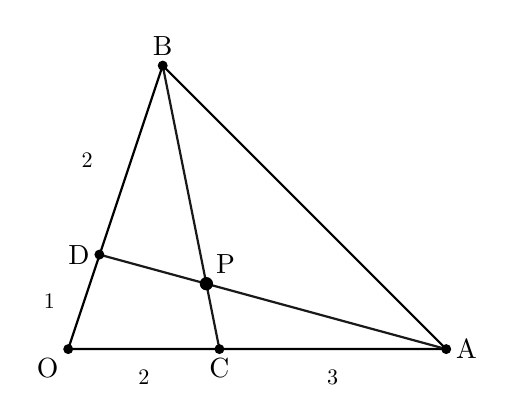
\begin{tikzpicture}[scale=1.2]
    \coordinate (O) at (0,0);
    \coordinate (A) at (4, 0);
    \coordinate (B) at (1, 3);
    
    % C on OA (2:3) -> 2/5 of OA
    \coordinate (C) at (1.6, 0);
    % D on OB (1:2) -> 1/3 of OB
    \coordinate (D) at (0.33, 1);
    
    \draw[thick] (O)--(A)--(B)--cycle;
    \draw[thick, mainBlack] (A)--(D);
    \draw[thick, mainBlack] (B)--(C);
    
    \path[name path=AD] (A)--(D);
    \path[name path=BC] (B)--(C);
    \path[name intersections={of=AD and BC, by=P}];
    
    \fill (O) circle (1.5pt) node[below left] {O};
    \fill (A) circle (1.5pt) node[right] {A};
    \fill (B) circle (1.5pt) node[above] {B};
    \fill (C) circle (1.5pt) node[below] {C};
    \fill (D) circle (1.5pt) node[left] {D};
    \fill (P) circle (2pt) node[above right] {P};
    
    \node[scale=0.8] at (0.8, -0.3) {2}; \node[scale=0.8] at (2.8, -0.3) {3};
    \node[scale=0.8] at (-0.2, 0.5) {1}; \node[scale=0.8] at (0.2, 2) {2};
\end{tikzpicture}
\end{center}

\talk{私}{「まず、AD上の点として考えてみよう。PはADを $s : (1-s)$ に内分する点と置けるはずだ」}

\begin{align*}
    \overrightarrow{\text{OP}} &= (1-s)\overrightarrow{\text{OA}} + s\overrightarrow{\text{OD}} \\
    &= (1-s)\vec{a} + s\left(\frac{1}{3}\vec{b}\right) \quad \cdots \text{\ajMaru{1}}
\end{align*}

\talk{友人}{「次はBC上の点としてだね。$t : (1-t)$ と置けばいいかな」}

\begin{align*}
    \overrightarrow{\text{OP}} &= t\overrightarrow{\text{OC}} + (1-t)\overrightarrow{\text{OB}} \\
    &= t\left(\frac{2}{5}\vec{a}\right) + (1-t)\vec{b} \quad \cdots \text{\ajMaru{2}}
\end{align*}

\talk{先生}{「\ajMaru{1}と\ajMaru{2}は、同じ矢印 $\overrightarrow{\text{OP}}$ を別の言い方で表したものです。ベクトルの世界では、分解の一意性(住所はただ一つ)がありましたね」}
\talk{友人}{「そうか! $\vec{a}$ の係数同士、$\vec{b}$ の係数同士が、完全に一致しないといけないんだ」}

\talk{私}{(係数比較……。連立方程式に持ち込めば、未知数 $s, t$ が求まる!)}

\newpage

% -------------------------------------------------------
% 4ページ目:解答とエピローグ
% -------------------------------------------------------
\subsection*{Solve: 運命の交差点を特定する}

私たちは連立方程式を解き始めた。

\[
\begin{cases}
    1-s = \frac{2}{5}t & (\vec{a}\text{の係数}) \\
    \frac{1}{3}s = 1-t & (\vec{b}\text{の係数})
\end{cases}
\]

\talk{私}{「下の式から $t = 1 - \frac{1}{3}s$ だね。これを上の式に代入しよう」}
\[ 1-s = \frac{2}{5}\left( 1 - \frac{1}{3}s \right) \]
\[ 15 - 15s = 6 - 2s \implies 13s = 9 \implies s = \frac{9}{13} \]

\talk{友人}{「$s$ が出た! じゃあこれを \ajMaru{1} の式に戻せば……」}
\[ \overrightarrow{\text{OP}} = \left( 1 - \frac{9}{13} \right)\vec{a} + \frac{1}{3} \cdot \frac{9}{13}\vec{b} \]
\[ \overrightarrow{\text{OP}} = \frac{4}{13}\vec{a} + \frac{3}{13}\vec{b} \]

\talk{先生}{「正解です。これで交点Pの位置が、$\vec{a}, \vec{b}$ という基本の言葉だけで記述できました」}

\begin{SolidBox}
    \textbf{解答のポイント}
    \begin{enumerate}
        \item 交点Pを「2つの直線の上の点」として2通りに表す。
        \item 「係数の和が1」の形(内分点の公式)を使うとスムーズ。
        \item 一次独立の呪文($\vec{a} \neq \vec{0}, \vec{b} \neq \vec{0}, \vec{a} \not\parallel \vec{b}$)を唱えて、係数を比較する。
    \end{enumerate}
\end{SolidBox}

\vspace{1em}
\hrule
\vspace{1em}

\subsection*{Epilogue: 交差する運命}

問題を解き終えると、窓の外はすっかり暗くなっていた。
空にはオリオン座が昇っている。3つの星が、見事に一直線に並んでいる。

\talk{私}{「『係数の和が1』……。ただの計算ルールだと思ってたけど、こうやって使うと、点がそのライン上にいるための『縛り』に見えてくるね」}
\talk{友人}{「うん。PはADの縛りとBCの縛りを両方受けてて、その両方を満たすギリギリの場所があの一点だったんだね」}

\talk{先生}{「その通り。連立方程式を解くということは、複数の運命(条件)が交差する一点を見つけ出す作業なのです」}

先生は夜空を見上げた。

\talk{先生}{「さて、今回は真面目に連立方程式を解きましたが、実はもっとズルい……いえ、賢い近道もあります。図形の比率だけを一瞬で見抜く魔法、\textbf{『メネラウスの定理』}です。次回はそれを使ってみましょう」}

\vspace{2em}
\begin{flushright}
    \textit{To be continued in Lecture 9...}
\end{flushright}

% =======================================================
% 第9回
% =======================================================
\setcounter{section}{8} % 第9回
\setKey{Crossing Paths}

\section{交差する運命 —— 交点の位置ベクトル}

% -------------------------------------------------------
% 1ページ目:プロローグと基本戦略
% -------------------------------------------------------
\subsection*{Prologue: 森の中の十字路}

黒板には大きな三角形と、その内部で交差する2本の線が描かれている。
先生はチョークを置き、私たちに向き直った。

\talk{先生}{「深い森の中で、二つの獣道が交差しているとします。その『交差点』の場所を、地図上で正確に指し示すにはどうすればいいでしょう?」}
\talk{友人}{「GPSがあれば一発だけど……」}
\talk{先生}{「文明の利器がない場合は? 私たちにあるのは、始点Oからのベクトルというロープと、基本的な計算力だけです」}

私は黒板の交点Pをじっと見る。Pは、一方の道の上にもあるし、もう一方の道の上にもある。

\talk{私}{(……交差点Pは、道Aの住人でもあり、道Bの住人でもある。二重国籍みたいなものかな)}

\talk{私}{「点Pは2つの直線の上にあるから、両方の条件を満たす場所……ってことですよね」}
\talk{先生}{「その通り。Pは\textbf{二つの顔(所属)}を持っています。その二重スパイのような性質を利用して、Pの正体(位置ベクトル)を暴くのです」}

\vspace{1em}
\hrule
\vspace{2em}

\subsection{Topic 1: 二つの住所を突き合わせる}

先生は具体的な問題を書き出した。ベクトルの応用問題として最も有名な「交点の位置ベクトル」だ。

\begin{NoteBox}
    \textbf{例題:交点の位置ベクトル} \\
    $\triangle$OAB において、辺OAを $5:2$ に内分する点をC、辺OBを $2:1$ に内分する点をDとする。
    線分ADと線分BCの交点をPとするとき、$\overrightarrow{\text{OP}}$ を $\vec{a}, \vec{b}$ で表せ。
\end{NoteBox}

\begin{center}
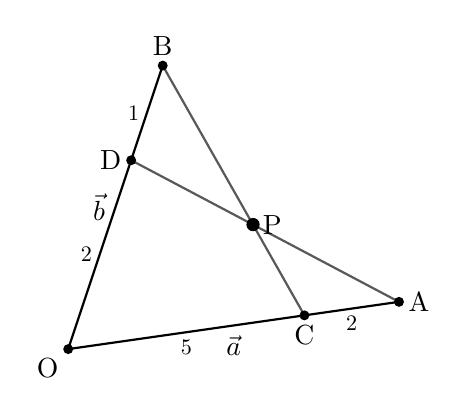
\begin{tikzpicture}[scale=1.2, >=stealth]
    \coordinate (O) at (0,0);
    \coordinate (A) at (3.5, 0.5);
    \coordinate (B) at (1, 3);
    
    % C on OA (5:2) -> 5/7
    \coordinate (C) at ($(O)!0.714!(A)$);
    % D on OB (2:1) -> 2/3
    \coordinate (D) at ($(O)!0.666!(B)$);
    
    % Intersection P
    \path[name path=AD] (A)--(D);
    \path[name path=BC] (B)--(C);
    \path[name intersections={of=AD and BC, by=P}];
    
    \draw[thick] (O)--(A) node[midway, below] {$\vec{a}$};
    \draw[thick] (O)--(B) node[midway, left] {$\vec{b}$};
    \draw[thick, subGray] (A)--(D);
    \draw[thick, subGray] (B)--(C);
    
    \fill (O) circle (1.5pt) node[below left] {O};
    \fill (A) circle (1.5pt) node[right] {A};
    \fill (B) circle (1.5pt) node[above] {B};
    \fill (C) circle (1.5pt) node[below] {C};
    \fill (D) circle (1.5pt) node[left] {D};
    \fill (P) circle (2pt) node[right] {P};
    
    \node[scale=0.8] at ($(O)!0.5!(C)$) [below] {5};
    \node[scale=0.8] at ($(C)!0.5!(A)$) [below] {2};
    \node[scale=0.8] at ($(O)!0.5!(D)$) [left] {2};
    \node[scale=0.8] at ($(D)!0.5!(B)$) [left] {1};
\end{tikzpicture}
\end{center}

\talk{先生}{「点Pの正体を暴くために、二人の証人に話を聞きましょう。まず、直線ADさん」}
\talk{友人}{「PはAD上にいるから……内分点の公式が使えるね。比率はわからないから、$s : (1-s)$ とおけばいいかな」}
\talk{先生}{「ええ。PはADを内分する点ですからね。ではもう一人、直線BCさんにも証言してもらいましょう」}
\talk{私}{「こっちは $t : (1-t)$ とおいて……二つの式が作れそうです」}

\newpage

% -------------------------------------------------------
% 2ページ目:係数比較法
% -------------------------------------------------------
\subsection{Solve: 連立方程式へ}

私たちはノートに式を書き始めた。

\begin{enumerate}
    \item \textbf{AD上の点としての証言:}
    Pは線分ADを $s : (1-s)$ に内分する。
    \[ \overrightarrow{\text{OP}} = (1-s)\overrightarrow{\text{OA}} + s\overrightarrow{\text{OD}} \]
    ここで $\overrightarrow{\text{OD}} = \frac{2}{3}\vec{b}$ なので、
    \[ \overrightarrow{\text{OP}} = (1-s)\vec{a} + \frac{2}{3}s\vec{b} \quad \cdots \text{\ajMaru{1}} \]
    
    \item \textbf{BC上の点としての証言:}
    Pは線分BCを $t : (1-t)$ に内分する。
    \[ \overrightarrow{\text{OP}} = (1-t)\overrightarrow{\text{OB}} + t\overrightarrow{\text{OC}} \]
    ここで $\overrightarrow{\text{OC}} = \frac{5}{7}\vec{a}$ なので、
    \[ \overrightarrow{\text{OP}} = \frac{5}{7}t\vec{a} + (1-t)\vec{b} \quad \cdots \text{\ajMaru{2}} \]
\end{enumerate}

\talk{先生}{「\ajMaru{1}と\ajMaru{2}は、表現は違いますが全く同じ矢印 $\overrightarrow{\text{OP}}$ を指しています。ここで、あの\textbf{『呪文』}の出番ですよ」}
\talk{友人}{「えっと……『$\vec{a} \neq \vec{0}, \vec{b} \neq \vec{0}, \vec{a} \not\parallel \vec{b}$ なので』だっけ?」}
\talk{先生}{「正解。一次独立であることの宣言です。これがあれば、係数を比較して連立方程式を作ることができます」}

\talk{私}{「$\vec{a}$ の係数同士、$\vec{b}$ の係数同士が、完全に一致しないといけないんですね」}

\[
\begin{cases}
    1-s = \frac{5}{7}t & (\vec{a}\text{の係数}) \\
    \frac{2}{3}s = 1-t & (\vec{b}\text{の係数})
\end{cases}
\]

\talk{私}{(あとはこれを解くだけだ。計算ミスしないように慎重に……)}

下の式から $t = 1 - \frac{2}{3}s$。これを上の式に代入する。
\[ 1-s = \frac{5}{7}\left( 1 - \frac{2}{3}s \right) \]
\[ 1-s = \frac{5}{7} - \frac{10}{21}s \]
\[ 1 - \frac{5}{7} = s - \frac{10}{21}s \]
\[ \frac{2}{7} = \frac{11}{21}s \]
\[ s = \frac{2}{7} \times \frac{21}{11} = \frac{6}{11} \]

\talk{友人}{「$s$ が出た! $6/11$ だね。じゃあこれを \ajMaru{1} の式に戻せば……」}

\[ \overrightarrow{\text{OP}} = \left( 1 - \frac{6}{11} \right)\vec{a} + \frac{2}{3} \cdot \frac{6}{11}\vec{b} \]
\[ \overrightarrow{\text{OP}} = \frac{5}{11}\vec{a} + \frac{4}{11}\vec{b} \]

\talk{先生}{「お見事。これで交点Pの位置が、$\vec{a}, \vec{b}$ という基本の言葉だけで記述できました」}

\begin{SolidBox}
    \textbf{解法のポイント(係数比較法)}
    \begin{enumerate}
        \item 交点を「2つの直線の上の点」として、2通りの式で表す。
        \item 「係数の和が1」の形(内分点の公式)を使うとスムーズ。
        \item 一次独立の条件を確認し、連立方程式を解く。
    \end{enumerate}
\end{SolidBox}

\newpage

% -------------------------------------------------------
% 3ページ目:メネラウスの定理
% -------------------------------------------------------
\subsection{Topic 2: 幾何の近道(メネラウスの定理)}

計算を終えて一息ついていると、先生がニヤリと笑った。

\talk{先生}{「素晴らしい計算力です。……が、もし『検算』や『答えだけ』が欲しいなら、森の抜け道がありますよ」}
\talk{私}{「抜け道?」}
\talk{先生}{「連立方程式を解かずに、図形の比率を一瞬で見抜く魔法。\textbf{メネラウスの定理}です」}

先生は黒板の図形の上を、キツネのような動きで指でなぞった。

\begin{SolidBox}
    \textbf{定理:メネラウスの定理(Menelaus' Theorem)} \\
    三角形と、それを横切る直線について、
    頂点$\to$分点$\to$頂点$\dots$と一筆書きで回ると、比の積が1になる。
    \[ \frac{\text{頂}}{\text{分}} \times \frac{\text{分}}{\text{頂}} \times \frac{\text{頂}}{\text{分}} = 1 \]
\end{SolidBox}

\begin{center}
\begin{tikzpicture}[scale=1.0, >=stealth]
    \coordinate (O) at (0,0);
    \coordinate (A) at (3,0);
    \coordinate (B) at (1,2);
    \coordinate (C) at (2,0); % on OA
    \coordinate (D) at (0.5,1); % on OB
    \coordinate (P) at (intersection of A--D and B--C);
    
    \draw[thick] (O)--(A)--(B)--cycle;
    \draw[thick, dashed] (A)--(D);
    \draw[thick, dashed] (B)--(C);
    
    \node[below] at (O) {O}; \node[below] at (A) {A}; \node[above] at (B) {B};
    \node[below] at (C) {C}; \node[left] at (D) {D}; \node[right] at (P) {P};
    
    % Path
    \draw[->, thick, subGray] (O) to[bend left] (D);
    \draw[->, thick, subGray] (D) to[bend left] (B);
    \draw[->, thick, subGray] (B) to[bend left] (P);
    \draw[->, thick, subGray] (P) to[bend left] (C);
    \draw[->, thick, subGray] (C) to[bend left] (A);
    \draw[->, thick, subGray] (A) to[bend left] (O);
    
    \node[align=center] at (4,1) {$\triangle$OAD と直線BC\\ について考える};
\end{tikzpicture}
\end{center}

\talk{友人}{「えっ、これで $s$ が求まるの?」}
\talk{先生}{「やってみましょう。$\triangle$OAD と直線BC(分断線)に注目してください」}

\[ \frac{OD}{DB} \times \frac{BP}{PC} \times \frac{CA}{AO} = 1 \]
ではなく、求めたい比(AP:PD)を含むルートを選びます。$\triangle$OCP と直線 AD……いや、$\triangle$OAD と直線 BPC ですね。

\talk{先生}{「$\triangle$OADを一筆書きします。O $\to$ B $\to$ D $\to$ P $\to$ A $\to$ C $\to$ O の順です」}

\[ \frac{OB}{BD} \times \frac{DP}{PA} \times \frac{AC}{CO} = 1 \]

条件より $OD:DB=2:1$ なので $OB:BD=3:1$。
$OC:CA=5:2$ なので $AC:CO=2:5$。

\[ \frac{3}{1} \times \frac{DP}{PA} \times \frac{2}{5} = 1 \]
\[ \frac{6}{5} \times \frac{DP}{PA} = 1 \implies \frac{DP}{PA} = \frac{5}{6} \]

\talk{私}{「$DP:PA = 5:6$……つまり $AP:PD = 6:5$! さっき出した $s = \frac{6}{11}$ と一致します!」}
\talk{友人}{「うわ、方程式なしで比率が出ちゃった。これを使えば計算ミスも防げそうだね」}

\newpage

% -------------------------------------------------------
% 4ページ目:エピローグ
% -------------------------------------------------------
\subsection*{Epilogue: 複数の地図を持つこと}

\talk{私}{「代数的に解く(連立方程式)のと、幾何的に解く(メネラウス)。同じ山を登るのに、全然違うルートがあるんですね」}
\talk{先生}{「その通り。代数は力技ですが、どんな道でも切り開けます。幾何は閃きが必要ですが、驚くほど近道ができます。両方の地図を持っておくことが、遭難しない秘訣ですよ」}

私はノートを見返す。
びっしりと書かれた連立方程式の横に、シンプルなメネラウスの図。
どちらも同じ「真理」にたどり着いているのが、なんだか面白い。

\talk{先生}{「さて、これで平面上の位置は自由自在に扱えるようになりました。次回は、さらに世界を広げましょう。ベクトルの『内積』を使って、円を描いたり、直線を引いたり……\textbf{図形の方程式}の世界へと進みます」}

\talk{友人}{「図形の方程式? $y=ax+b$ みたいな?」}
\talk{先生}{「ええ。でもベクトルを使えば、もっと直感的で、美しい式になりますよ」}

\vspace{2em}
\begin{flushright}
    \textit{To be continued in Lecture 10...}
\end{flushright}

\newpage

% =======================================================
% 第10回
% =======================================================
\setcounter{section}{9} % 第10回
\setKey{The Misleading Name}

\section{動く矢印の軌跡 —— ベクトル方程式(直線)}

% -------------------------------------------------------
% 1ページ目:プロローグ(方程式の定義)
% -------------------------------------------------------
\subsection*{Prologue: 名前への違和感}

放課後の図書室。友人が教科書を開いたまま、腕組みをして唸っている。

\talk{友人}{「納得いかない」}
\talk{私}{「何が?」}
\talk{友人}{「この\textbf{『ベクトル方程式』}って名前だよ。方程式って言ったらさ、$3x+5=14$ みたいに『解(答え)』を求めるものでしょ? でもここに出てくる式は、解くわけじゃなくて図形を表すっていうじゃん」}

私は友人の言葉に同意する。確かに、私たちはこれまで「$x$ を求めよ」という命令に慣れすぎていた。

\talk{私}{(方程式=解くもの。その固定観念があるから、図形の式を見たときに『で、何をすればいいの?』って戸惑うんだ)}

先生が本を抱えて通りかかった。

\talk{先生}{「ふふ、なるほど。言葉の定義に敏感なのは数学の才能がある証拠ですよ」}
d\talk{先生}{「確かに中学までの『方程式』は『未知数を見つけるための鍵』でした。しかし、これからの『方程式(Equation)』は意味が変わります。それは\textbf{『条件』}であり、その条件を満たす点たちの\textbf{『会員証』}なのです」}

\vspace{1em}
\hrule
\vspace{2em}

\subsection{Topic 1: 静止画から動画へ}

先生は黒板に一本の直線を引いた。

\talk{先生}{「直線とは何でしょう? 点の集まりですね。では、どんな点が集まれば直線になるのか。それをベクトルの言葉で記述してみましょう」}

\talk{私}{「直線を引くために必要なものは……『通る点A』と『進む向き』かな」}
\talk{先生}{「その通り。点A($\vec{a}$) から出発して、ある方向 $\vec{d}$ に向かって歩いていく様子を想像してください」}

\begin{SolidBox}
    \textbf{直線のベクトル方程式(方向ベクトル型)} \\
    点 A($\vec{a}$) を通り、方向ベクトル $\vec{d}$ に平行な直線上の任意の点 P($\vec{p}$) は、実数 $t$ を用いて次のように表される。
    \[ \vec{p} = \vec{a} + t\vec{d} \]
\end{SolidBox}

\talk{友人}{「$\vec{a}$ まで行って、そこから $t$ 倍の $\vec{d}$ を足す……。うん、これなら意味が分かる。でも先生、これって『方程式』っぽくないよ。ただの足し算の式じゃん」}
\talk{先生}{「鋭いですね。実はこれは『パラメータ表示』と呼ばれる形式です。$t$ という時間を動かすことで、点Pが直線上をスーッと動いていく動画のようなイメージですね」}

\begin{center}
\begin{tikzpicture}[scale=1.0, >=stealth]
    \coordinate (O) at (0,0);
    \coordinate (A) at (1,1);
    \coordinate (D) at (2,1); % direction
    \coordinate (P) at (4,2.5); % t=1.5
    
    % Line
    \draw[dashed, gray] (-0.5, 0.25) -- (5, 3);
    
    % Vectors
    \draw[->, thick, subGray] (O) -- (A) node[midway, left] {$\vec{a}$};
    \draw[->, very thick, mainBlack] (A) -- (P) node[midway, above left] {$t\vec{d}$};
    \draw[->, thick, mainBlack] (O) -- (P) node[midway, right] {$\vec{p}$};
    
    \fill (O) circle (1.5pt) node[below left] {O};
    \fill (A) circle (1.5pt) node[above left] {A};
    \fill (P) circle (2pt) node[above] {P};
    
    \node[draw, fill=white, inner sep=2pt] at (3, 0.5) {$t$ が変わると P が動く};
\end{tikzpicture}
\end{center}

\talk{私}{($t=1$ なら1時間後の場所、$t=-1$ なら1時間前の場所。$t$ があらゆる値をとることで、点Pの軌跡が『直線』として浮かび上がるわけか)}

\newpage

% -------------------------------------------------------
% 2ページ目:法線ベクトル
% -------------------------------------------------------
\subsection{Topic 2: 拒絶のルール(法線ベクトル)}

\talk{先生}{「では、もう一つ。直線を定義する全く異なる方法を紹介しましょう。道を歩くのではなく、\textbf{『通せんぼ』}をするのです」}
\talk{私}{「通せんぼ?」}
\talk{先生}{「ある点Aを通る、ベクトル $\vec{n}$ に\textbf{垂直}な直線、と考えてください。この $\vec{n}$ を\textbf{法線(ほうせん)ベクトル}といいます」}

先生は黒板に、直線に対して直角に突き刺さる矢印を描いた。

\talk{先生}{「直線上のどんな点Pをとっても、ベクトル $\overrightarrow{\text{AP}}$ は、常に法線 $\vec{n}$ と垂直になりますね。垂直といえば?」}
\talk{友人}{「あ、前回やった……\textbf{内積がゼロ}!」}

\begin{SolidBox}
    \textbf{直線のベクトル方程式(法線ベクトル型)} \\
    点 A($\vec{a}$) を通り、法線ベクトル $\vec{n}$ に垂直な直線上の点 P($\vec{p}$) は、次の等式を満たす。
    \[ \vec{n} \cdot (\vec{p} - \vec{a}) = 0 \]
\end{SolidBox}

\begin{center}
\begin{tikzpicture}[scale=1.0, >=stealth]
    \coordinate (O) at (0,-0.5);
    \coordinate (A) at (2,1);
    \coordinate (P) at (3.5,0); % P on the line
    \coordinate (N) at (3,2.5); % Normal vector direction
    
    % Line (Perpendicular to AN)
    \draw[thick, borderGray] (0.5, 2) -- (4.5, -0.66);
    
    % Vectors
    \draw[->, thick, subGray] (O) -- (A) node[midway, left] {$\vec{a}$};
    \draw[->, thick, subGray] (O) -- (P) node[midway, below] {$\vec{p}$};
    \draw[->, very thick, mainBlack] (A) -- (P) node[midway, below left] {$\vec{p}-\vec{a}$};
    \draw[->, very thick, mainBlack] (A) -- (N) node[midway, right] {$\vec{n}$ (法線)};
    
    % Right angle mark
    \pic [draw, angle radius=3mm] {right angle = P--A--N};
    
    \fill (O) circle (1.5pt) node[below left] {O};
    \fill (A) circle (1.5pt) node[above left] {A};
    \fill (P) circle (2pt) node[below] {P};
\end{tikzpicture}
\end{center}

\talk{友人}{「おお、これなら『方程式(=0)』っぽい! 『$\vec{n}$ と垂直であれ』っていう命令を感じる」}
\talk{私}{「『進む方向』を指定しなくても、『進んではいけない方向(垂直方向)』を指定すれば、道は決まるわけですね」}

\vspace{1em}
\hrule
\vspace{2em}

\subsection{Topic 3: 係数の正体}

\talk{先生}{「この法線ベクトルの式を成分で計算すると、驚くべき事実が見えてきます。$\vec{n}=(a, b)$、A$(x_1, y_1)$、P$(x, y)$ としましょう」}

私たちはノートで計算を始めた。
\[ \vec{n} \cdot (\vec{p} - \vec{a}) = 0 \]
\[ (a, b) \cdot (x-x_1, y-y_1) = 0 \]
\[ a(x-x_1) + b(y-y_1) = 0 \]
\[ ax + by - ax_1 - by_1 = 0 \]

\talk{私}{「定数部分($-ax_1-by_1$)をまとめて $c$ と置くと…… $ax + by + c = 0$ になります!」}
\talk{先生}{「そうです。これは中学・高校で何度も見た『直線の一般形』ですね。では、この式の $x$ と $y$ の係数 $(a, b)$ は、一体何を表していたのでしょう?」}

\talk{友人}{「えっ……まさか、法線ベクトル?」}
\talk{先生}{「その通りです」}

\begin{NoteBox}
    \textbf{係数の幾何学的意味} \\
    直線の方程式 $ax + by + c = 0$ における係数のベクトル $\vec{n} = (a, b)$ は、その直線の\textbf{法線ベクトル(垂直なベクトル)}を表している。
\end{NoteBox}

\talk{私}{(衝撃だ。今まで $3x+4y+5=0$ を見て『ただの数式だな』としか思ってなかったけど、実は『$(3, 4)$ という矢印に垂直になれ!』っていう図形的な命令だったのか……)}

\newpage

% -------------------------------------------------------
% 3ページ目:演習
% -------------------------------------------------------
\subsection*{Check: 視点を変えて解く}

\begin{NoteBox}
    \textbf{問題} \\
    点 $A(2, 3)$ を通り、直線 $2x - 3y + 1 = 0$ に\textbf{垂直}な直線の方程式を求めよ。
\end{NoteBox}

\talk{友人}{「えっと、今までのやり方だと……元の直線の傾きが $2/3$ だから、垂直な直線の傾きは $-3/2$ で……」}
\talk{先生}{「それでも解けますが、法線ベクトルを使うともっと速いですよ」}

\talk{私}{「やってみます。元の直線 $2x - 3y + 1 = 0$ の法線ベクトルは $\vec{n} = (2, -3)$ です」}
\talk{友人}{「求める直線は、これに『垂直』なんだよね? ってことは、求める直線の法線ベクトルはどうなるの?」}

私は図を描いて考える。元の直線の法線 $\vec{n}$ は、元の直線に垂直だ。
求める直線は、元の直線に垂直だ。
……ということは、求める直線は $\vec{n}$ と\textbf{平行}になる!

\talk{私}{「いや、待てよ。もっと単純に考えよう。求める直線の『方向ベクトル』が $(2, -3)$ になるってことか」}
\talk{先生}{「正解。あるいは、求める直線の『法線ベクトル』は、$(2, -3)$ に垂直なベクトル……つまり $(3, 2)$ だと考えてもいいですね」}

\talk{友人}{「法線が $(3, 2)$ なら、式の形は $3x + 2y + c = 0$ になるはず!」}
\talk{私}{「あとは点 $A(2, 3)$ を通るから、代入して $3(2) + 2(3) + c = 0 \implies 12 + c = 0 \implies c = -12$」}

\[ \text{答え:} \quad 3x + 2y - 12 = 0 \]

\talk{先生}{「お見事。傾きの計算をしなくても、ベクトルの成分を入れ替えるだけで直線の概形が決まってしまう。これがベクトルの効用です」}

\vspace{1em}
\hrule
\vspace{2em}

\subsection*{Epilogue: 静と動の境界}

\talk{私}{「今まで $y=2x+1$ とか見ても、ただの数式としか思ってませんでした。でもベクトルを通すと、それが『方向』や『垂直』といった意味を持って動き出すんですね」}
\talk{先生}{「ええ。方程式(Equation)とは、静止した等式ではありません。条件を満たす点たちが織りなす、ダイナミックな軌跡なのです」}

先生は黒板の図形にチョークで円を描き加えた。

\talk{先生}{「直線が描けるなら、円も描けるはずです。次回は、コンパスの動きをベクトルで記述してみましょう。円のベクトル方程式です」}

\vspace{1em}
\begin{flushright}
    \textit{To be continued in Lecture 11...}
\end{flushright}

\newpage

% =======================================================
% 第11回
% =======================================================
\setcounter{section}{10} % 第11回
\setKey{The Perfect Constraint}

\section{距離による支配 —— 円のベクトル方程式}

% -------------------------------------------------------
% 1ページ目:プロローグと基本形
% -------------------------------------------------------
\subsection*{Prologue: 繋がれた犬}

昼休み、校庭の隅にある木に、リードで繋がれた犬がいる。
犬は走り回ろうとするが、ピンと張ったリードがそれを許さない。

\talk{友人}{「あーあ、行きたいところに行けなくて不満そうだね」}
\talk{私}{「でも、あのリードがあるおかげで、行動範囲がはっきりしてるよな。中心(木)から半径(リードの長さ)以内のエリアしか動けない」}

その時、先生が通りかかり、私たちの視線を追った。

\talk{先生}{「彼は不自由に見えて、実は非常に美しい数学的対象を描いています。彼がリードをピンと張って走り回るとき、その軌跡は完璧な\textbf{円}になりますからね」}
\talk{友人}{「円かぁ。コンパスで描くやつだね」}
\talk{先生}{「そうです。円とは『ある一点から等距離にある点の集合』です。このシンプルな\textbf{距離の制約(Constraint)}を、ベクトルの言葉で書き下してみましょう」}

\vspace{1em}
\hrule
\vspace{2em}

\subsection{Topic 1: 基本形(中心と半径)}

教室に戻り、先生は黒板に点C(Center)と、そこから距離 $r$ だけ離れた点Pを描いた。

\talk{先生}{「中心 C($\vec{c}$) からの距離が常に $r$ である点 P($\vec{p}$)。この条件を数式に翻訳するとどうなりますか?」}
\talk{私}{「距離はベクトルの大きさだから…… $\overrightarrow{\text{CP}}$ の大きさが $r$ ってことですよね」}

\begin{SolidBox}
    \textbf{円のベクトル方程式(基本形)} \\
    中心 C($\vec{c}$), 半径 $r$ の円の方程式は
    \[ |\vec{p} - \vec{c}| = r \]
\end{SolidBox}

\talk{私}{(絶対値がつくと難しそうに見えるけど、意味は『CとPの距離』ってだけなんだな。シンプルだ)}

\talk{先生}{「意味はこれで完璧です。しかし、実際に計算するときに絶対値は邪魔ですよね。どうしますか?」}
\talk{友人}{「2乗する! 前にやった『殻を破る』やつだね」}

\begin{align*}
    |\vec{p} - \vec{c}|^2 &= r^2 \\
    (\vec{p} - \vec{c}) \cdot (\vec{p} - \vec{c}) &= r^2
\end{align*}

\talk{先生}{「その通り。計算問題では、この\textbf{内積の形}にしてから成分を代入したり、展開したりするのが定石です」}

\begin{center}
\begin{tikzpicture}[scale=1.0, >=stealth]
    \coordinate (O) at (0, -0.5);
    \coordinate (C) at (2, 1.5);
    \def\rad{1.5}
    
    % Circle
    \draw[thick, subGray] (C) circle (\rad);
    \fill (C) circle (1.5pt) node[below] {C($\vec{c}$)};
    \fill (O) circle (1.5pt) node[below left] {O};
    
    % Vectors
    \draw[->, thick, subGray] (O) -- (C);
    
    % P
    \coordinate (P) at ($(C) + (45:\rad)$);
    \draw[->, thick, mainBlack] (O) -- (P) node[midway, left] {$\vec{p}$};
    \fill (P) circle (2pt) node[above right] {P};
    
    % Radius vector
    \draw[->, very thick, mainBlack] (C) -- (P) node[midway, above left] {$\vec{p}-\vec{c}$};
    \node[right] at (3.5, 2.5) {長さが一定 ($r$)};
\end{tikzpicture}
\end{center}

\newpage

% -------------------------------------------------------
% 2ページ目:直径形
% -------------------------------------------------------
\subsection{Topic 2: 直径形(直角の利用)}

\talk{先生}{「円にはもう一つ、有名な定義がありましたね。中学校で習った『タレスの定理』を覚えていますか?」}
\talk{友人}{「えっと……半円の弧に対する円周角は90度、だっけ?」}
\talk{先生}{「正解。直径を見込む角は直角になります。これを使えば、中心や半径がわからなくても、\textbf{直径の両端}だけで円を記述できます」}

先生は黒板に2点A, Bを描き、それを直径とする円を描いた。円周上のどこに点Pを取っても、$\angle APB$ は直角になる。

\talk{私}{「直角……つまり、垂直ってことか。ベクトルで垂直といえば?」}
\talk{友人}{「内積がゼロ!」}

\begin{SolidBox}
    \textbf{円のベクトル方程式(直径形)} \\
    2点 A($\vec{a}$), B($\vec{b}$) を直径の両端とする円の方程式は
    \[ (\vec{p} - \vec{a}) \cdot (\vec{p} - \vec{b}) = 0 \]
    ($\overrightarrow{\text{AP}} \perp \overrightarrow{\text{BP}}$ または PがA, Bと一致)
\end{SolidBox}

\begin{center}
\begin{tikzpicture}[scale=1.0, >=stealth]
    \coordinate (A) at (0, 0);
    \coordinate (B) at (4, 0);
    \coordinate (C) at (2, 0);
    \coordinate (P) at (3, 1.732); % on circle
    
    \draw[subGray] (C) circle (2);
    \draw[thick] (A) -- (B);
    \fill (A) circle (1.5pt) node[left] {A($\vec{a}$)};
    \fill (B) circle (1.5pt) node[right] {B($\vec{b}$)};
    \fill (P) circle (2pt) node[above] {P($\vec{p}$)};
    
    \draw[->, thick, mainBlack] (A) -- (P) node[midway, left] {$\overrightarrow{\text{AP}}$};
    \draw[->, thick, mainBlack] (B) -- (P) node[midway, right] {$\overrightarrow{\text{BP}}$};
    
    \pic [draw, angle radius=3mm] {right angle = A--P--B};
    
    \node[below] at (2, -0.5) {内積ゼロ $\iff$ 垂直};
\end{tikzpicture}
\end{center}

\talk{私}{「この形、すごくシンプルですね。中心も半径も出てこない」}
\talk{先生}{「でも、展開して整理すればちゃんと中心が出てきますよ。試しに展開してみましょうか」}

\begin{align*}
    (\vec{p} - \vec{a}) \cdot (\vec{p} - \vec{b}) &= 0 \\
    |\vec{p}|^2 - \vec{p}\cdot\vec{b} - \vec{a}\cdot\vec{p} + \vec{a}\cdot\vec{b} &= 0 \\
    |\vec{p}|^2 - (\vec{a}+\vec{b})\cdot\vec{p} + \vec{a}\cdot\vec{b} &= 0
\end{align*}

\talk{先生}{「これを平方完成のように変形すると、中心が $\frac{\vec{a}+\vec{b}}{2}$、つまり\textbf{中点}であることが見えてきます」}

\talk{私}{(なるほど。式変形だけで、幾何学的な事実(中心は中点)が導き出されるんだ。数式は嘘をつかないな)}

\newpage

% -------------------------------------------------------
% 3ページ目:垂直二等分線
% -------------------------------------------------------
\subsection{Topic 3: 公平な境界線(垂直二等分線)}

\talk{先生}{「さて、少し視点を変えましょう。もし点Pが、一点に縛られるのではなく、\textbf{二つの点 A, B から等距離}にあるとしたら?」}
\talk{友人}{「あっちに行ったりこっちに来たり……真ん中の線になるかな」}
\talk{先生}{「そう、垂直二等分線です。式で書くとどうなりますか?」}

\begin{SolidBox}
    \textbf{垂直二等分線のベクトル方程式} \\
    2点 A($\vec{a}$), B($\vec{b}$) からの距離が等しい点 P($\vec{p}$) の軌跡
    \[ |\vec{p} - \vec{a}| = |\vec{p} - \vec{b}| \]
\end{SolidBox}

\talk{私}{「これ、両辺を2乗したらどうなるんだろう。円のときは $|\vec{p}|^2$ が残ったけど……」}

私はノートで計算を試みる。

\begin{align*}
    |\vec{p} - \vec{a}|^2 &= |\vec{p} - \vec{b}|^2 \\
    |\vec{p}|^2 - 2\vec{p}\cdot\vec{a} + |\vec{a}|^2 &= |\vec{p}|^2 - 2\vec{p}\cdot\vec{b} + |\vec{b}|^2
\end{align*}

\talk{私}{「あ! 両辺にある $|\vec{p}|^2$ が消える!」}
\talk{先生}{「そこが重要です。2次の項が消えて1次の項(内積)だけが残る。だから\textbf{直線}になるのです。逆に、2次の項が消えなければ……?」}

\subsection{Topic 4: 歪んだ鏡(アポロニウスの円)}

\talk{先生}{「もし距離の比が $1:1$ じゃなかったらどうでしょう。例えば、Aからの距離がBからの距離の2倍だとしたら?」}
\talk{友人}{「えっと、$|\vec{p}-\vec{a}| = 2|\vec{p}-\vec{b}|$ ってこと?」}

\talk{私}{「これ、2乗しても $|\vec{p}|^2$ の係数が揃わないぞ。左辺は1倍だけど、右辺は4倍になるから……」}
\[ |\vec{p}|^2 - \dots = 4(|\vec{p}|^2 - \dots) \]
\[ 3|\vec{p}|^2 - \dots = 0 \]

\talk{私}{「$|\vec{p}|^2$ が消えずに残る! ってことは……」}
\talk{先生}{「そう、また\textbf{円}に戻るのです。これを\textbf{アポロニウスの円}と呼びます」}

\begin{NoteBox}
    \textbf{アポロニウスの円} \\
    2点 A, B からの距離の比が $m:n$ ($m \neq n$) である点の軌跡は円になる。
    (線分ABを $m:n$ に内分する点と外分する点を直径の両端とする円)
\end{NoteBox}

\begin{center}
\begin{tikzpicture}[scale=0.8, >=stealth]
    \coordinate (A) at (0,0);
    \coordinate (B) at (3,0);
    
    % Circle for 2:1 ratio
    % Internal: 2:1 -> 2/3 of 3 = 2 -> (2,0) relative to A. Wait.
    % A at 0, B at 3.
    % p such that |p| = 2|p-3|. p^2 = 4(p-3)^2 ...
    % Let's just draw schematically
    \draw[dashed] (-1,0) -- (6,0);
    \fill (A) circle (2pt) node[below] {A};
    \fill (B) circle (2pt) node[below] {B};
    
    % Circle
    \draw[thick, subGray] (4,0) circle (2);
    \node at (4, -2.5) {Bに近い側の領域を囲む円になる};
    
    \fill (2,0) circle (2pt) node[below left] {内分};
    \fill (6,0) circle (2pt) node[below right] {外分};
\end{tikzpicture}
\end{center}

\talk{友人}{「へええ。比が $1:1$ のときだけ直線になって、バランスが崩れると円になって相手を囲い込んじゃうんだ。なんか人間関係みたいだね」}
\talk{先生}{「面白い解釈ですね。数式は正直です。力の均衡が崩れれば、世界は歪み、閉じた円環になるのです」}

\newpage

% -------------------------------------------------------
% 4ページ目:エピローグ
% -------------------------------------------------------
\subsection*{Epilogue: 制約が生む形}

チャイムが鳴る。

\talk{私}{「$|\vec{p}-\vec{c}|=r$ なら円。$|\vec{p}-\vec{a}| = |\vec{p}-\vec{b}|$ なら直線。式の形を見ただけで、その図形が持つ『性質』が見えてきました」}
\talk{先生}{「素晴らしい。絶対値がついているからといって、計算する前にビビる必要はありません。その式が何を意味しているか、翻訳すればいいのです」}

先生は黒板を消しながら言った。

\talk{先生}{「次回は、これまで学んだベクトル方程式——直線、円、存在範囲——を総動員して、演習問題に挑みましょう。アポロニウスの円も、実際に計算して確かめてみますよ」}

\vspace{1em}
\begin{flushright}
    \textit{To be continued in Lecture 12...}
\end{flushright}

\newpage

% =======================================================
% 第12回
% =======================================================
\setcounter{section}{11} % 第12回
\setKey{The Art of Translation}

\section{翻訳の技法 —— ベクトル方程式演習}

% -------------------------------------------------------
% 1ページ目:プロローグ(暗号解読)
% -------------------------------------------------------
\subsection*{Prologue: 暗号を解く者}

放課後の教室。黒板には、先生が書いた数式が一つだけ残されている。
\[ (\vec{p} - \vec{a}) \cdot (\vec{p} - \vec{b}) = 0 \]

先生は私たちの方を向き、試すような目で問いかけた。

\talk{先生}{「数学とは、ある種の言語です。この式を見たとき、君たちはどう反応しますか? ただの計算問題として展開し始めますか? それとも、そこにある『意味』を読み取りますか?」}
\talk{私}{「展開……したくなっちゃうかな。$|\vec{p}|^2 - (\vec{a}+\vec{b})\cdot\vec{p} + \dots$ って感じで」}
\talk{友人}{「でもそれじゃ、計算が大変になるだけだよ。この式は『内積がゼロ』って言ってるんだから……」}

友人は黒板の前に歩み寄り、チョークで図を描き始めた。2点A, Bと、その周りにある点P。

\talk{友人}{「ほら、$\overrightarrow{\text{AP}} \cdot \overrightarrow{\text{BP}} = 0$ ってことだよね。AからPへの矢印と、BからPへの矢印が垂直になる場所。……これ、円だよね?」}
\talk{先生}{「正解です。直径ABを見込む角は直角。だからこれは、線分ABを直径とする円を表しています」}

私は友人の描いた図と、数式を見比べる。
ただの記号の羅列に見えていた式が、急に具体的な形を持って浮かび上がってきた。

\talk{私}{(なるほど。式変形をする前に、式の『意味』を翻訳すれば、計算なしで図形の形が見えてくるのか。まるで外国語の翻訳みたいだ)}

\talk{先生}{「今日は、無機質な数式を豊かな図形のイメージに翻訳する練習——\textbf{ベクトル方程式の解読}を行いましょう」}

\vspace{1em}
\hrule
\vspace{2em}

\subsection{Topic 1: 直線と円の文法}

\talk{先生}{「まずは基本文法の復習です。直線と円、それぞれの『型』を思い出してください」}

\begin{SolidBox}
    \textbf{翻訳ガイド:直線の型}
    \begin{itemize}
        \item \textbf{方向ベクトル型} $\vec{p} = \vec{a} + t\vec{d}$ \\
        $\to$ 「Aを通って、$\vec{d}$ 方向に進む道」
        \item \textbf{法線ベクトル型} $\vec{n} \cdot (\vec{p} - \vec{a}) = 0$ \\
        $\to$ 「Aを通って、$\vec{n}$ に垂直な壁」
    \end{itemize}
\end{SolidBox}

\begin{SolidBox}
    \textbf{翻訳ガイド:円の型}
    \begin{itemize}
        \item \textbf{基本形} $|\vec{p} - \vec{c}| = r$ \\
        $\to$ 「中心Cから距離 $r$ の結界」
        \item \textbf{直径形} $(\vec{p} - \vec{a}) \cdot (\vec{p} - \vec{b}) = 0$ \\
        $\to$ 「直径ABを見込む直角の軌跡」
    \end{itemize}
\end{SolidBox}

\talk{先生}{「では、少しひねった問題を読んでみましょう」}

\begin{NoteBox}
    \textbf{例題1:式の読み取り} \\
    次の方程式はどのような図形を表すか。
    \[ (\vec{p} + \vec{a}) \cdot (\vec{p} - \vec{a}) = 0 \]
\end{NoteBox}

\talk{私}{「内積がゼロだから、円かな? でも $\vec{p}+\vec{a}$ って何だろう」}
\talk{友人}{「$\vec{p} - (-\vec{a})$ と書き直せばいいんじゃない? そうすれば『点 $-\vec{a}$ から P へのベクトル』になるよ」}
\talk{私}{「そうか! つまり、点A($\vec{a}$) と 点A'($-\vec{a}$) を直径の両端とする円だ」}
\talk{先生}{「その通り。ちなみに展開すると $|\vec{p}|^2 - |\vec{a}|^2 = 0 \iff |\vec{p}| = |\vec{a}|$ となり、原点中心の円であることが分かります」}

\newpage

% -------------------------------------------------------
% 2ページ目:接線の方程式
% -------------------------------------------------------
\subsection{Topic 2: 拒絶する壁(円の接線)}

\talk{先生}{「次は新しい翻訳です。円の\textbf{接線}をベクトルで表してみましょう」}

先生は黒板に円を描き、その上の一点 $\text{P}_0(\vec{p}_0)$ で接する直線を引いた。

\talk{先生}{「円の接線には、非常に重要な幾何学的性質があります。中心Cと接点$\text{P}_0$を結ぶ半径は、接線とどういう関係にありますか?」}
\talk{友人}{「垂直に交わるよね。接線は半径に対して直角だ」}
\talk{先生}{「そう。つまり、接線とは\textbf{『点$\text{P}_0$を通り、半径ベクトル $\overrightarrow{\text{CP}_0}$ に垂直な直線』}のことなのです」}

私はその言葉を聞いて、直線の「法線ベクトル型」を思い出した。
通る点と、垂直なベクトル。必要なパーツは揃っている。

\talk{私}{(あ! それって直線の『法線ベクトル型』がそのまま使えるってことか。半径 $\vec{n} = \overrightarrow{\text{CP}_0}$ を、そのまま法線ベクトルとして採用すればいいんだ)}

\talk{私}{「つまり、半径ベクトルを法線ベクトル $\vec{n}$ だと思えばいいんですね」}
\talk{先生}{「ご名答。式を立ててみましょう」}

\begin{SolidBox}
    \textbf{円の接線のベクトル方程式} \\
    中心 C($\vec{c}$) の円上の点 $\text{P}_0(\vec{p}_0)$ における接線は、
    法線ベクトル $\vec{n} = \vec{p}_0 - \vec{c}$ を用いて次のように書ける。
    \[ \vec{n} \cdot (\vec{p} - \vec{p}_0) = 0 \]
    \[ (\vec{p}_0 - \vec{c}) \cdot (\vec{p} - \vec{p}_0) = 0 \]
\end{SolidBox}

\begin{center}
\begin{tikzpicture}[scale=1.0, >=stealth]
    \coordinate (O) at (0,-0.5);
    \coordinate (C) at (1,1);
    \coordinate (P0) at (2.5, 1.8); % on circle roughly
    \coordinate (P) at (2.9, 1.0); % on tangent line
    
    % Circle
    \draw[thick, subGray] (C) circle (1.7);
    \fill (C) circle (1.5pt) node[left] {C};
    \fill (P0) circle (2pt) node[above left] {$\text{P}_0(\vec{p}_0)$};
    \fill (P) circle (2pt) node[right] {P($\vec{p}$)};
    
    % Radius (Normal)
    \draw[->, thick, mainBlack] (C) -- (P0) node[midway, above] {$\vec{n}$};
    
    % Tangent Line
    \draw[thick, mainBlack] ($(P0)!1.5!90:(C)$) -- ($(P0)!1.5!-90:(C)$);
    
    % Vector on line
    \draw[->, thick, subGray] (P0) -- (P) node[midway, below right] {$\vec{p}-\vec{p}_0$};
    
    \pic [draw, angle radius=3mm] {right angle = C--P0--P};
    
    \node[align=left, draw=borderGray, fill=white] at (4, 2.5) {半径がそのまま\\法線になる!};
\end{tikzpicture}
\end{center}

\talk{友人}{「公式を覚える必要ないね。『半径と垂直』ってことだけ分かってれば、その場で作れる」}
\talk{先生}{「それが大事なのです。公式を暗記するのではなく、図形の構造を理解していれば、いつでも式は再現できます」}

\vspace{1em}
\hrule
\vspace{2em}

\subsection{Topic 3: 軌跡の翻訳(アポロニウスの円)}

\talk{先生}{「最後は少し手強い翻訳です。次の式を見てください」}

\[ |\vec{p} - \vec{a}| = 2|\vec{p} - \vec{b}| \]

\talk{私}{「距離の式ですね。Aからの距離が、Bからの距離の2倍?」}
\talk{友人}{「あっちに行ったりこっちに行ったり……どこになるんだろう」}

\talk{先生}{「直感でわからなければ、計算の力(代数)を借りましょう。絶対値を外すには?」}
\talk{私}{「2乗します!」}

\begin{align*}
    |\vec{p} - \vec{a}|^2 &= 4|\vec{p} - \vec{b}|^2 \\
    |\vec{p}|^2 - 2\vec{p}\cdot\vec{a} + |\vec{a}|^2 &= 4(|\vec{p}|^2 - 2\vec{p}\cdot\vec{b} + |\vec{b}|^2)
\end{align*}

\talk{私}{「整理すると $3|\vec{p}|^2 - \dots = 0$ となって、$|\vec{p}|^2$ の項が残っちゃいます。直線なら消えるはずなのに」}
\talk{先生}{「2次の項があるということは……」}
\talk{友人}{「あ、\textbf{円}だ!」}
\talk{先生}{「そう。これを\textbf{アポロニウスの円}と呼びます」}

\newpage

% -------------------------------------------------------
% 3ページ目:アポロニウスの円と垂直二等分線
% -------------------------------------------------------
\subsection*{Study: 距離の比と図形の形}

\talk{先生}{「距離の比 $AP:BP = m:n$ において、比率が変わると図形がどう変わるか見てみましょう」}

\begin{SolidBox}
    \textbf{距離の比による軌跡の分類} \\
    条件:$n|\vec{p} - \vec{a}| = m|\vec{p} - \vec{b}|$ \quad ($AP:BP = m:n$)
    \begin{itemize}
        \item \textbf{$m = n$ のとき:} ($1:1$) \\
        $|\vec{p} - \vec{a}| = |\vec{p} - \vec{b}|$ \\
        $\implies$ \textbf{垂直二等分線}(直線)
        \item \textbf{$m \neq n$ のとき:} \\
        $\implies$ \textbf{アポロニウスの円}
    \end{itemize}
\end{SolidBox}

\talk{友人}{「$1:1$ のときだけ直線になるんだね。なんで?」}
\talk{先生}{「2乗して計算したとき、両辺の係数が同じなら $|\vec{p}|^2$ が消えてなくなるからです。2次の項が消えれば、残るのは1次の項(直線)だけですよね」}

\begin{center}
\begin{tikzpicture}[scale=0.8, >=stealth]
    \coordinate (A) at (0,0);
    \coordinate (B) at (3,0);
    
    \draw[dashed] (-1,0) -- (6,0);
    \fill (A) circle (2pt) node[below] {A};
    \fill (B) circle (2pt) node[below] {B};
    
    % Bisector (1:1)
    \draw[thick, subGray] (1.5, -2) -- (1.5, 2) node[above] {$1:1$ (直線)};
    
    % Circle
    \draw[thick, mainBlack] (5.33, 0) circle (1.33);
    \node at (5.33, -1.8) {近い方を囲む円};
    
    \node[align=left] at (1.5, -2.5) {力の均衡が崩れると、\\弱い方(距離が近い方)を\\囲い込む円になる};
\end{tikzpicture}
\end{center}

\talk{私}{「なるほど。力が等しければ真っ直ぐな境界線だけど、片方が強すぎると空間が歪んで、相手を囲い込んじゃうのか」}
\talk{友人}{「人間関係みたいで怖いね」}

\subsection*{Check: 軌跡を特定せよ}

\begin{NoteBox}
    \textbf{問題} \\
    $|\vec{p} + 2\vec{a}| = |\vec{p} - 4\vec{a}|$ を満たす点 P($\vec{p}$) はどのような図形を描くか。
\end{NoteBox}

\talk{私}{「係数がどちらも1倍だから、$|\vec{p}|^2$ は消えるはず。つまり直線だね」}
\talk{友人}{「式の意味を翻訳しよう。左辺は $|\vec{p} - (-2\vec{a})|$ だから、点 $-2\vec{a}$ からの距離」}
\talk{私}{「右辺は 点 $4\vec{a}$ からの距離。その二つが等しいってことは……」}

\talk{先生}{「答えが見えましたか?」}
\talk{二人}{「\textbf{線分を結ぶ垂直二等分線}です!」}

\vspace{1em}
\hrule
\vspace{1em}

\subsection*{Epilogue: 翻訳家の眼}

\talk{先生}{「数式は、一見すると無味乾燥な記号の列です。しかし、ベクトルの言葉を知っていれば、そこには鮮やかな図形が浮かび上がってきます」}
\talk{私}{「$|\vec{p}-\vec{a}|=|\vec{p}-\vec{b}|$ が、ただの計算式ではなく、二つの点の間を走る公平な境界線に見えてきました」}

手元のノートを見返す。かつては意味不明な記号に見えていた方程式が、今は「円」や「直線」という形を伴って語りかけてくるようだ。

\talk{私}{(翻訳家の眼……か。その眼を持てば、僕たちはもう計算の奴隷じゃない。図形の支配者になれるのかもしれないな)}

先生は窓の外を指さした。

\talk{先生}{「さて、これで直交座標の世界での話は一通り終わりました。次回は、最後のフロンティア。マス目が歪んだ世界——\textbf{存在範囲(斜交座標)}——へと足を踏み入れましょう」}

\vspace{1em}
\begin{flushright}
    \textit{To be continued in Lecture 13...}
\end{flushright}

% --- 解答 ---
\newpage
\section*{Appendix: 演習問題の解答}

\begin{SolidBox}
    \textbf{例題1の解答}
    
    方程式:$(\vec{p} + \vec{a}) \cdot (\vec{p} - \vec{a}) = 0$
    
    式変形すると:
    \[ (\vec{p} - (-\vec{a})) \cdot (\vec{p} - \vec{a}) = 0 \]
    
    これは、2点 $\vec{a}, -\vec{a}$ を直径の両端とする円を表す。
    (中心は原点O、半径 $|\vec{a}|$ の円)
\end{SolidBox}

\vspace{1em}

\begin{SolidBox}
    \textbf{Check問題の解答}
    
    方程式:$|\vec{p} - (-2\vec{a})| = |\vec{p} - 4\vec{a}|$
    
    これは、2点 $\mathbf{-2\vec{a}}$ と $\mathbf{4\vec{a}}$ からの距離が等しい点の集合である。
    
    よって求める図形は、
    \textbf{2点 $-2\vec{a}, 4\vec{a}$ を結ぶ線分の垂直二等分線}。
    
    (補足:この線分の中点は $\frac{-2\vec{a}+4\vec{a}}{2} = \vec{a}$ なので、点A($\vec{a}$)を通り、ベクトル $\vec{a}$ に垂直な直線となる)
\end{SolidBox}

\newpage
% =======================================================
% 第13回(最終回)
% =======================================================
\setcounter{section}{12} % 第13回
\setKey{The Distorted Grid}

\section{歪んだグリッド —— 存在範囲}

% -------------------------------------------------------
% 1ページ目:プロローグ(動く係数)
% -------------------------------------------------------
\subsection*{Prologue: 塗り絵のルール}

最終回の授業。先生は黒板に大きな平行四辺形の網目(グリッド)を描いている。
第2回で見た「斜めのマス目」だ。

\talk{先生}{「これまで私たちは、特定の点(定点)を扱ってきました。しかし今日は、点を動かして『面』を塗ってみましょう」}
\talk{友人}{「面を塗る? ベクトルで?」}
\talk{先生}{「ええ。基本式はいつも通りです」}

\[ \vec{p} = s\vec{a} + t\vec{b} \]

\talk{先生}{「この $s$ と $t$ が、ある範囲で動くとき、点Pはどんな足跡を残すのか。それが今日のテーマ\textbf{『存在範囲』}です」}

私は手元のノートに、$\vec{a}$ と $\vec{b}$ を描いてみる。
$s=1, t=1$ なら平行四辺形の対角線の先っちょだ。$s=0.5, t=0.5$ なら……ちょうど真ん中あたりかな。

\talk{私}{(係数 $s, t$ は、言わば『座標』だ。$(s, t)$ が動けば、点Pも地図の上を動く。問題は、どんなルールで動くかだね)}

\vspace{1em}
\hrule
\vspace{2em}

\subsection{Topic 1: 直線への回帰}

\talk{先生}{「まずは復習から。点Pが『直線AB上』にあるための条件は何でしたか?」}
\talk{友人}{「係数の和が1! $s + t = 1$ だよね」}
\talk{先生}{「その通りです。予算が合計100万円($s+t=1$)あって、それを $\vec{a}$ と $\vec{b}$ に振り分けるイメージでしたね」}

\begin{SolidBox}
    \textbf{直線の存在範囲} \\
    \[ \vec{p} = s\vec{a} + t\vec{b}, \quad s + t = 1 \]
    $\implies$ 点Pは\textbf{直線AB}を描く。
\end{SolidBox}

\talk{私}{「$s+t=1$ というルールがある限り、点Pは直線ABというレールから外れられない。……ここまでは今まで通りだ」}

\begin{center}
\begin{tikzpicture}[scale=1.0, >=stealth]
    \coordinate (O) at (0,0);
    \coordinate (A) at (3,0.5);
    \coordinate (B) at (1,2);
    
    \draw[->, thick, subGray] (O)--(A) node[below] {$\vec{a}$};
    \draw[->, thick, subGray] (O)--(B) node[left] {$\vec{b}$};
    
    % 修正:AとBを通るように自動計算して延長(前後0.5倍分延長)
    \draw[thick, mainBlack] ($(A)!-0.5!(B)$) -- ($(B)!-0.5!(A)$) node[left] {直線AB ($s+t=1$)};
    
    \fill (A) circle (1.5pt) node[right] {A(1,0)};
    \fill (B) circle (1.5pt) node[above] {B(0,1)};
\end{tikzpicture}
\end{center}

\newpage

% -------------------------------------------------------
% 2ページ目:三角形の領域
% -------------------------------------------------------
\subsection{Topic 2: 境界の内側(三角形)}

\talk{先生}{「では、ルールを少し緩めましょう。予算が『ちょうど100万円』ではなく、『100万円\textbf{以内}』だとしたら?」}

\[ s + t \leqq 1, \quad s \geqq 0, \quad t \geqq 0 \]

\talk{友人}{「ぴったり1なら直線AB上だったけど……少なくなってもいいんだよね。$s=0.1, t=0.1$ とか」}
\talk{私}{「それだと、原点Oのすぐ近くだね。$s=0, t=0$ なら原点そのものだし」}

私は図の中の点をいくつか打ってみる。
直線ABよりも「手前(原点側)」の点なら、どれも $s+t < 1$ になりそうだ。

\talk{私}{(……そうか。直線ABが『限界ライン』なんだ。そのラインの内側にあるエリア全部が、許された場所になる)}

\talk{私}{「先生、これって\textbf{三角形OABの内部}(周も含む)になりますか?」}
\talk{先生}{「正解です。$s \geqq 0, t \geqq 0$ という条件は、マイナス方向(逆走)はダメという意味。つまり、$\vec{a}$ と $\vec{b}$ に挟まれたエリアの中で、さらに限界ラインの内側ということになります」}

\begin{SolidBox}
    \textbf{三角形の領域} \\
    \[ \vec{p} = s\vec{a} + t\vec{b}, \quad s + t \leqq 1, \quad s \geqq 0, \ t \geqq 0 \]
    $\implies$ $\mathbf{\triangle OAB}$ \textbf{の周および内部}
\end{SolidBox}

\begin{center}
\begin{tikzpicture}[scale=1.0, >=stealth]
    \coordinate (O) at (0,0);
    \coordinate (A) at (3,0.5);
    \coordinate (B) at (1,2);
    
    \draw[->, thick, mainBlack] (O)--(A) node[below] {$\vec{a}$};
    \draw[->, thick, mainBlack] (O)--(B) node[left] {$\vec{b}$};
    
    \fill[gray!20] (O)--(A)--(B)--cycle;
    \draw[thick, mainBlack] (A)--(B);
    
    \node at (1.5, 0.8) {$s+t \leqq 1$};
    \node at (1.8, 1.2) {限界ラインの内側};
\end{tikzpicture}
\end{center}

\vspace{1em}
\hrule
\vspace{2em}

\subsection{Topic 3: 独立した自由(平行四辺形)}

\talk{先生}{「次は予算制をやめます。$s$ と $t$ がお互いに干渉せず、勝手に動けるとしたらどうでしょう?」}

\[ 0 \leqq s \leqq 1, \quad 0 \leqq t \leqq 1 \]

\talk{友人}{「足して1とか関係ないんだね。$s$ は0から1まで好きに動く。$t$ も好きに動く」}
\talk{私}{「$x$座標と$y$座標がそれぞれ範囲指定された感じかな。直交座標なら長方形になるけど、ここは歪んだ世界だから……」}

\talk{私}{($\vec{a}$ 方向に1まで、$\vec{b}$ 方向に1まで。網目を塗りつぶしていくと……\textbf{平行四辺形}になるはずだ)}

\begin{SolidBox}
    \textbf{平行四辺形の領域} \\
    \[ 0 \leqq s \leqq 1, \quad 0 \leqq t \leqq 1 \]
    $\implies$ O, A, B, $\text{C}(\vec{a}+\vec{b})$ を頂点とする\textbf{平行四辺形の周と内部}
\end{SolidBox}

\newpage

% -------------------------------------------------------
% 3ページ目:変形テクニック
% -------------------------------------------------------
\subsection{Topic 4: 基準を作り変える(変数変換)}

\talk{先生}{「では、本日のメインイベント。ちょっと意地悪な条件を出しますよ」}

\begin{NoteBox}
    \textbf{例題:} 次の条件を満たす点Pの存在範囲を図示せよ。
    \[ \vec{p} = s\vec{a} + t\vec{b}, \quad 2s + 3t \leqq 6, \quad s \geqq 0, \ t \geqq 0 \]
\end{NoteBox}

\talk{友人}{「うわ、右辺が $6$ だし、係数もバラバラ。これじゃ『足して1』が使えないよ」}
\talk{私}{「とりあえず右辺を $1$ にしたいね。両辺を $6$ で割ってみようか」}

\[ \frac{2s}{6} + \frac{3t}{6} \leqq 1 \iff \frac{s}{3} + \frac{t}{2} \leqq 1 \]

\talk{私}{「うーん、足して1の形にはなったけど、変数が $s/3$ と $t/2$ になっちゃった。これどう扱えばいいんだろう」}
\talk{先生}{「その変数を、新しい係数 $s', t'$ だと思ってしまえばいいのです」}

先生は黒板で鮮やかな式変形を見せた。

\[ \vec{p} = s\vec{a} + t\vec{b} = \frac{s}{3}(3\vec{a}) + \frac{t}{2}(2\vec{b}) \]

\talk{私}{「あ! 無理やり $s/3$ と $t/2$ を作ったのか。その代わり、後ろのベクトルが $3\vec{a}$ と $2\vec{b}$ に変わった!」}

\talk{先生}{「ここで、$s' = \frac{s}{3}, \ t' = \frac{t}{2}$ と置き換えてみましょう。条件式はどうなりますか?」}
\talk{友人}{「$s' + t' \leqq 1$ になる! しかも $s, t \geqq 0$ だから $s', t' \geqq 0$ もそのまま使えるね」}

\talk{私}{(なるほど……。係数が複雑なら、基準となるベクトル(基底)の方を伸び縮みさせて調整すればいいんだ。これはコロンブスの卵だね)}

\begin{SolidBox}
    \textbf{解答の指針}
    \begin{enumerate}
        \item 条件式の右辺を 1 にする。($\frac{s}{3} + \frac{t}{2} \leqq 1$)
        \item その分母に合わせて、ベクトルを変形する。$\frac{s}{3}(3\vec{a}) + \frac{t}{2}(2\vec{b})$
        \item 新しい基底 $3\vec{a}, 2\vec{b}$ を基準にした三角形を描く。
    \end{enumerate}
\end{SolidBox}

\begin{center}
\begin{tikzpicture}[scale=0.7, >=stealth]
    \coordinate (O) at (0,0);
    \coordinate (A) at (1.5,0);
    \coordinate (B) at (0.5,1);
    
    \coordinate (A3) at (4.5,0); % 3a
    \coordinate (B2) at (1,2);   % 2b
    
    % Original
    \draw[->, dashed, subGray] (O)--(A) node[below]{$\vec{a}$};
    \draw[->, dashed, subGray] (O)--(B) node[left]{$\vec{b}$};
    
    % Extended
    \draw[->, thick, mainBlack] (O)--(A3) node[below right]{$3\vec{a}$ (新しい基準)};
    \draw[->, thick, mainBlack] (O)--(B2) node[above left]{$2\vec{b}$ (新しい基準)};
    
    % Area
    \fill[gray!20] (O)--(A3)--(B2)--cycle;
    \draw[thick, mainBlack] (A3)--(B2);
    
    \node at (2, 1) {求める領域};
\end{tikzpicture}
\end{center}

\talk{私}{「つまり、元の $\triangle$OAB じゃなくて、もっと大きな三角形(OAを3倍、OBを2倍した点で作る三角形)の内部になるってことか」}
\talk{友人}{「面積でいうと……底辺3倍、高さ2倍だから、6倍だね!」}

\newpage

% -------------------------------------------------------
% 4ページ目:エピローグ(全体のまとめ)
% -------------------------------------------------------
\subsection*{Epilogue: 自由な地図をポケットに}

チャイムが鳴り、全13回の講義が終わった。
黒板には、私たちが描いた「歪んだグリッド」と「新しい三角形」が残っている。

\talk{先生}{「これで平面ベクトルの話はおしまいです。最初は『向きと大きさを持つ矢印』という単純な定義から始まりましたが、気づけば私たちは、この矢印を使って空間そのものを記述できるようになっていました」}

私はノートをパラパラと見返す。
ただの矢印だったものが、足し算で繋がり、内積で角度を語り、最後には領域を塗りつぶす絵筆になった。

\talk{私}{「最初は、座標がないと不安でした。でも今は、$\vec{a}$ と $\vec{b}$ さえあれば、どんな歪んだ世界でも迷わずに歩ける気がします」}
\talk{友人}{「僕はやっぱり、内積が好きかな。計算だけで直角が見つかるのが魔法みたいで楽しかった」}

先生は満足そうに頷き、愛用のチョークを置いた。

\talk{先生}{「世界は必ずしも直角(直交座標)ではありません。地図は一つではないのです。君たちがこれから出会う複雑な問題も、ベクトルという『自由な視点』を通せば、きっとシンプルな構造が見えてくるはずです」}

\talk{私}{(視点を変える、か。……うん、悪くない道具を手に入れたな)}

私は新しい地図をポケットにしまうように、ノートを閉じた。
教室の外には、どこまでも広がる自由な平面(セカイ)が待っている。

\vspace{3em}
\begin{center}
    {\Huge \textbf{Fin.}}
\end{center}

% =======================================================
% 裏表紙 (Back Cover)
% =======================================================
\newpage
\thispagestyle{empty}
\vspace*{\fill}

\begin{center}
    % --- アートワーク:ゼロ・ベクトル (Return to Origin) ---
    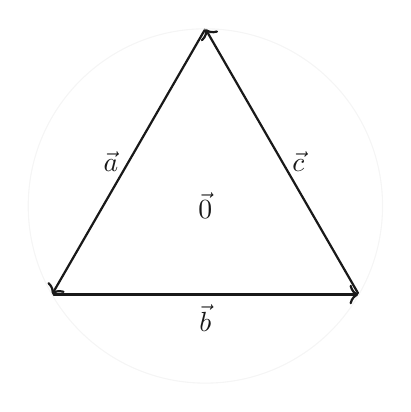
\begin{tikzpicture}[scale=1.5]
        % 3つのベクトルがループして元の位置に戻る(均衡と調和)
        \coordinate (O) at (0,0);
        \coordinate (A) at (90:1.5);
        \coordinate (B) at (210:1.5);
        \coordinate (C) at (330:1.5);
        
        \draw[->, thick, mainBlack] (A) -- (B) node[midway, left] {$\vec{a}$};
        \draw[->, thick, mainBlack] (B) -- (C) node[midway, below] {$\vec{b}$};
        \draw[->, thick, mainBlack] (C) -- (A) node[midway, right] {$\vec{c}$};
        
        % 中央のメッセージ
        \node[font=\sffamily\bfseries\color{mainBlack}] at (0,0) {$\vec{0}$};
        
        % 装飾の円(薄く)
        \draw[lightGray, thin] (0,0) circle (1.5);
    \end{tikzpicture}
    
    \vspace{3cm}
    
    % --- メッセージ ---
    \begin{minipage}{0.6\textwidth}
        \centering
        \sffamily \color{subGray} \small
        \textit{"The end of a journey is just another starting point."}
        \vspace{1em}
        
        \footnotesize
        旅の終わりは、ゼロに戻ることではない。\\
        それは、新たな始点に立つことだ。
    \end{minipage}

    \vspace{4cm}


\end{center}

\vspace*{\fill}

\end{document}